%\documentclass[sigconf,10pt]{acmart}
\documentclass[sigconf]{acmart}
\settopmatter{authorsperrow=4}
\settopmatter{printacmref=false}	% jin: remove ACM reference format box in the template
\renewcommand\footnotetextcopyrightpermission[1]{}

\pagenumbering{gobble}


\usepackage{verbatim}

\usepackage{listings}
\usepackage{url}            % simple URL typesetting

\usepackage{nicefrac}       % compact symbols for 1/2, etc.

%\usepackage{amsmath,amssymb,amsfonts}
\usepackage{algorithmic}

\usepackage{textcomp}
\usepackage{svg}
\usepackage{multirow}
\usepackage{tabularx}
\usepackage{graphics}
\usepackage{titlesec}


\lstset{frame=tb,
  language=python,
  aboveskip=3mm,
  belowskip=3mm,
  showstringspaces=false,
  columns=flexible,
  basicstyle={\small\ttfamily},
  numbers=none,
  captionpos=b,
  numberstyle=\tiny\color{gray},
  keywordstyle=\color{magenta},
  commentstyle=\color{blue},
  stringstyle=\color{magenta},
  breaklines=true,
  breakatwhitespace=true,
  tabsize=2
}

%\settopmatter{printfolios=false}		% -- Arup: no page numbers
%\renewcommand\footnotetextcopyrightpermission[1]{}

% Copyright
%\setcopyright{none}
%\setcopyright{acmcopyright}
%\setcopyright{acmlicensed}
%\setcopyright{rightsretained}
%\setcopyright{usgov}
%\setcopyright{usgovmixed}
%\setcopyright{cagov}
%\setcopyright{cagovmixed}

%\begin{comment}

\copyrightyear{2024}
\acmYear{2024}
\setcopyright{rightsretained}
\acmConference[Qualification Exam Defense]{Qualification Exam Defense}{December 6, 2:00 $\sim$ 3:00 pm, 2023}{Charlottesville VA, USA}
\acmBooktitle{Qualification Exam Defense
(Qualification Exam Defense), December 6, 2:00 $\sim$ 3:00 pm, 2023, Charlottesville VA, USA}
%\acmPrice{15.00}
%\acmDOI{10.1145/3576914.3587486}
%\acmISBN{979-8-4007-0049-1/23/05} %% Arup: Change it

%\end{comment}

%% DOI
%\acmDOI{10.475/123_4}
%
%% ISBN
%\acmISBN{123-4567-24-567/08/06}
%
%%Conference
%\acmConference[HOTMOBILE'22]{The 23nd International Workshop on Mobile Computing Systems and Applications}{Mar 2022}{Tempe, AZ}
%\acmYear{2022}
%\copyrightyear{2022}
%
%
%\acmArticle{4}
%\acmPrice{15.00}
%
%% These commands are optional
%%\acmBooktitle{Transactions of the ACM Woodstock conference}
%\editor{Jennifer B. Sartor}
%\editor{Theo D'Hondt}
%\editor{Wolfgang De Meuter}

%\input{header}
%\titlespacing*{\section}
%{0pt}{5.5ex plus 1ex minus .2ex}{4.3ex plus .2ex}

%\titlespacing*{\subsection}
%{0pt}{5.5ex plus 1ex minus .2ex}{4.3ex plus .2ex}

\begin{document}



\title{High-Performance Data Engineering on Amazon Web Services Using Python}
%\subtitle{Extended Abstract}
%\subtitlenote{The full version of the author's guide is available as
%  \texttt{acmart.pdf} document}
\author{Mills Wellons Staylor, III}
\email{qad5gv@virginia.edu}
\affiliation{
  \institution{University of Virginia}
  \country{USA}
}

%\author{Geoffrey Fox}
%\email{vxj6mb@virginia.edu}
%\affiliation{
%  \institution{University of Virginia}
%	\country{USA}
%}


% The default list of authors is too long for headers}
%\renewcommand{\shortauthors}{Arup et al.}

%
\begin{CCSXML}
<ccs2012>
<concept>
<concept_id>10010520.10010553.10010562.10010564</concept_id>
<concept_desc>AWS~Amazon Web Services/Cloud Computing</concept_desc>
<concept_significance>500</concept_significance>
</concept>
</ccs2012>
\end{CCSXML}

\ccsdesc[500]{Networks~Cloud Computing}
\ccsdesc[500]{FMI~Fast Messaging Interface}
\ccsdesc[500]{UCC~Unified Collective Communication}
\ccsdesc[500]{UCX~Unified Communication X}
\ccsdesc[500]{BSP~Bulk Synchronize Parallel}

%  https://doi.org/10.1145/3508396.3512875

\begin{abstract}
    \textbf{Data can be found everywhere, from health to human infrastructure to the surge of sensors to the proliferation of internet-linked devices. To meet this challenge, the data engineering domain has expanded monumentally in recent years in both research and industry.  Additionally, In recent years, the data engineering discipline has been dramatically impacted by Artificial Intelligence (AI) and Machine Learning (ML), which has resulted in research on the speed, performance, and optimization of such processes. Traditionally, data engineering, Machine Learning, and Artificial Intelligence workloads have been executed on large clusters in a data center environment.  This requires considerable investment in terms of both hardware and maintenance.  With the advent of the public cloud, it is now possible to run large applications across nodes without maintaining or owning hardware.  Serverless computing has emerged in cloud and open-source varieties to meet such needs.  This allows users of such systems to focus on the application code and take advantage of bundled CPUs and memory configuration without focusing primarily on the semantics of horizontal scalability and resource allocation. }

    \textbf{Serverless functions like AWS Lambda offer horizontal scaling and fine-grained billing.  However, when executing jobs or tasks on large datasets, users resort to low-cost or ephemeral storage options much slower than traditional HPC clusters.  To address this limitation, the FMI library has been developed and includes support for distributed collective operations such as direct, reduce, allreduce and scan using point-to-point communication. We detail specific results comparing Cylon and FMI on the AWS Cloud and UVA’s Rivanna supercomputer with the ultimate goal of developing a novel approach to deep learning training and inference on both cloud serverful and serverless environments and HPCs.   We will thoroughly explain FMI and Cylon's architecture and the execution process of Cylon tasks using Slurm, AWS ECS and AWS Step Functions. We show AWS Cylon and FMI achieve reasonable performance with minimal and constant overhead and compare these results to HPC clusters such as Rivanna Cylon.}

%The approach aims to excel in both scientific and engineering research HPC systems while demonstrating robust performance on cloud infrastructures. This dual capability fosters collaboration and innovation within the open-source scientific research community.

\end{abstract}

\maketitle
%\pagestyle{plain}

\section{Introduction and Motivation}\label{sec:intro}
The data engineering domain has expanded monumentally over the past decade, thanks to the emergence of Machine Learning (ML) and Artificial Intelligence (AI). Data is no longer categorized as Gigabytes (GB) or Megabytes (MB), files, or databases but as terabytes or abstract data stores. It takes a considerable amount of developer time for pre-processing when a better use of time would be designing and implementing deep learning or machine learning models. The increasing amount of connected internet devices and social media results in data growing at parabolic or exponential rates.  Therefore, improving performance is critical to continuing to build pipelines that support the development of optimized AI/ML training and inference.

The exponential growth in data volume and complexity poses significant challenges across various scientific domains, particularly in genomics, climate modeling, astronomy, and neuroscience. For instance, the 1000 Genomes project and the Cancer Genome Atlas alone utilize nearly five terabases of data\cite{McKenna2010The}. The TSE search terabase alone consumes a substantial 50.4 TB in size. This can be understood by considering that a single genome sequence alone can generate approximately 200 GB of data\cite{genomefaq:online}. Consequently, by 2025, it would be necessary to store the genome sequences of the entire world, amounting to a staggering 40 exabytes of storage.

Similar challenges exist in astronomy. Faaique (2024) highlights the difficulties associated with processing and analyzing astronomical data and proposes cloud computing and cloud storage as potential solutions\cite{faaique} due to the immense data size and scale involved. Fox and Fathkouhi (2024) further introduce AstroMAE, the first application of a Mask Encoder on astronomical data\cite{Fathkouhi2024}. This application utilizes a dataset comprising 659,857 images with a resolution of 64 × 64 pixels and five color bands, resulting in approximately 54 GB of data with 10.4 million learnable parameters.  Fox (2025) delves into the challenges astronomers face when attempting to execute inference on foundational models on large astronomical images using standalone devices. It highlights the limitations imposed by memory and resource constraints on such devices\cite{Staylor2024cosmic}.

Decomposing complex problems represented by large datasets can be challenging and demands both scalable and efficient solutions. Machine Learning and Artificial Intelligence have revolutionized data analysis, allowing researchers to extract valuable insights that were previously unattainable. This leads to more robust and reliable results than possible with the previously available tools.

A crucial aspect of these solutions is the use of analytical engines that run on High-Performance Computing (HPC) clusters for training Large Language Models (LLMs) \cite{abeykoon2020data}. However, a significant challenge with this approach is that frameworks like Pandas, NumPy, and PyTorch are not directly compatible with technologies such as MPI, UCC/UCX, or Open Fabric Interfaces (OFI). 

Between 2005 and 2015, JVM frameworks and languages revolutionized Big Data with sophisticated processing and analysis. Over the past decade, however, Python has seen increased adoption and usage, surpassing Java and JVM usage, according to Google Trends.  Figure \ref{fig:javapythonadoption} shows Java versus Pythons based on reported Google trends from 2019 to 2025.  

\begin{figure}[ht]
    \begin{center}
    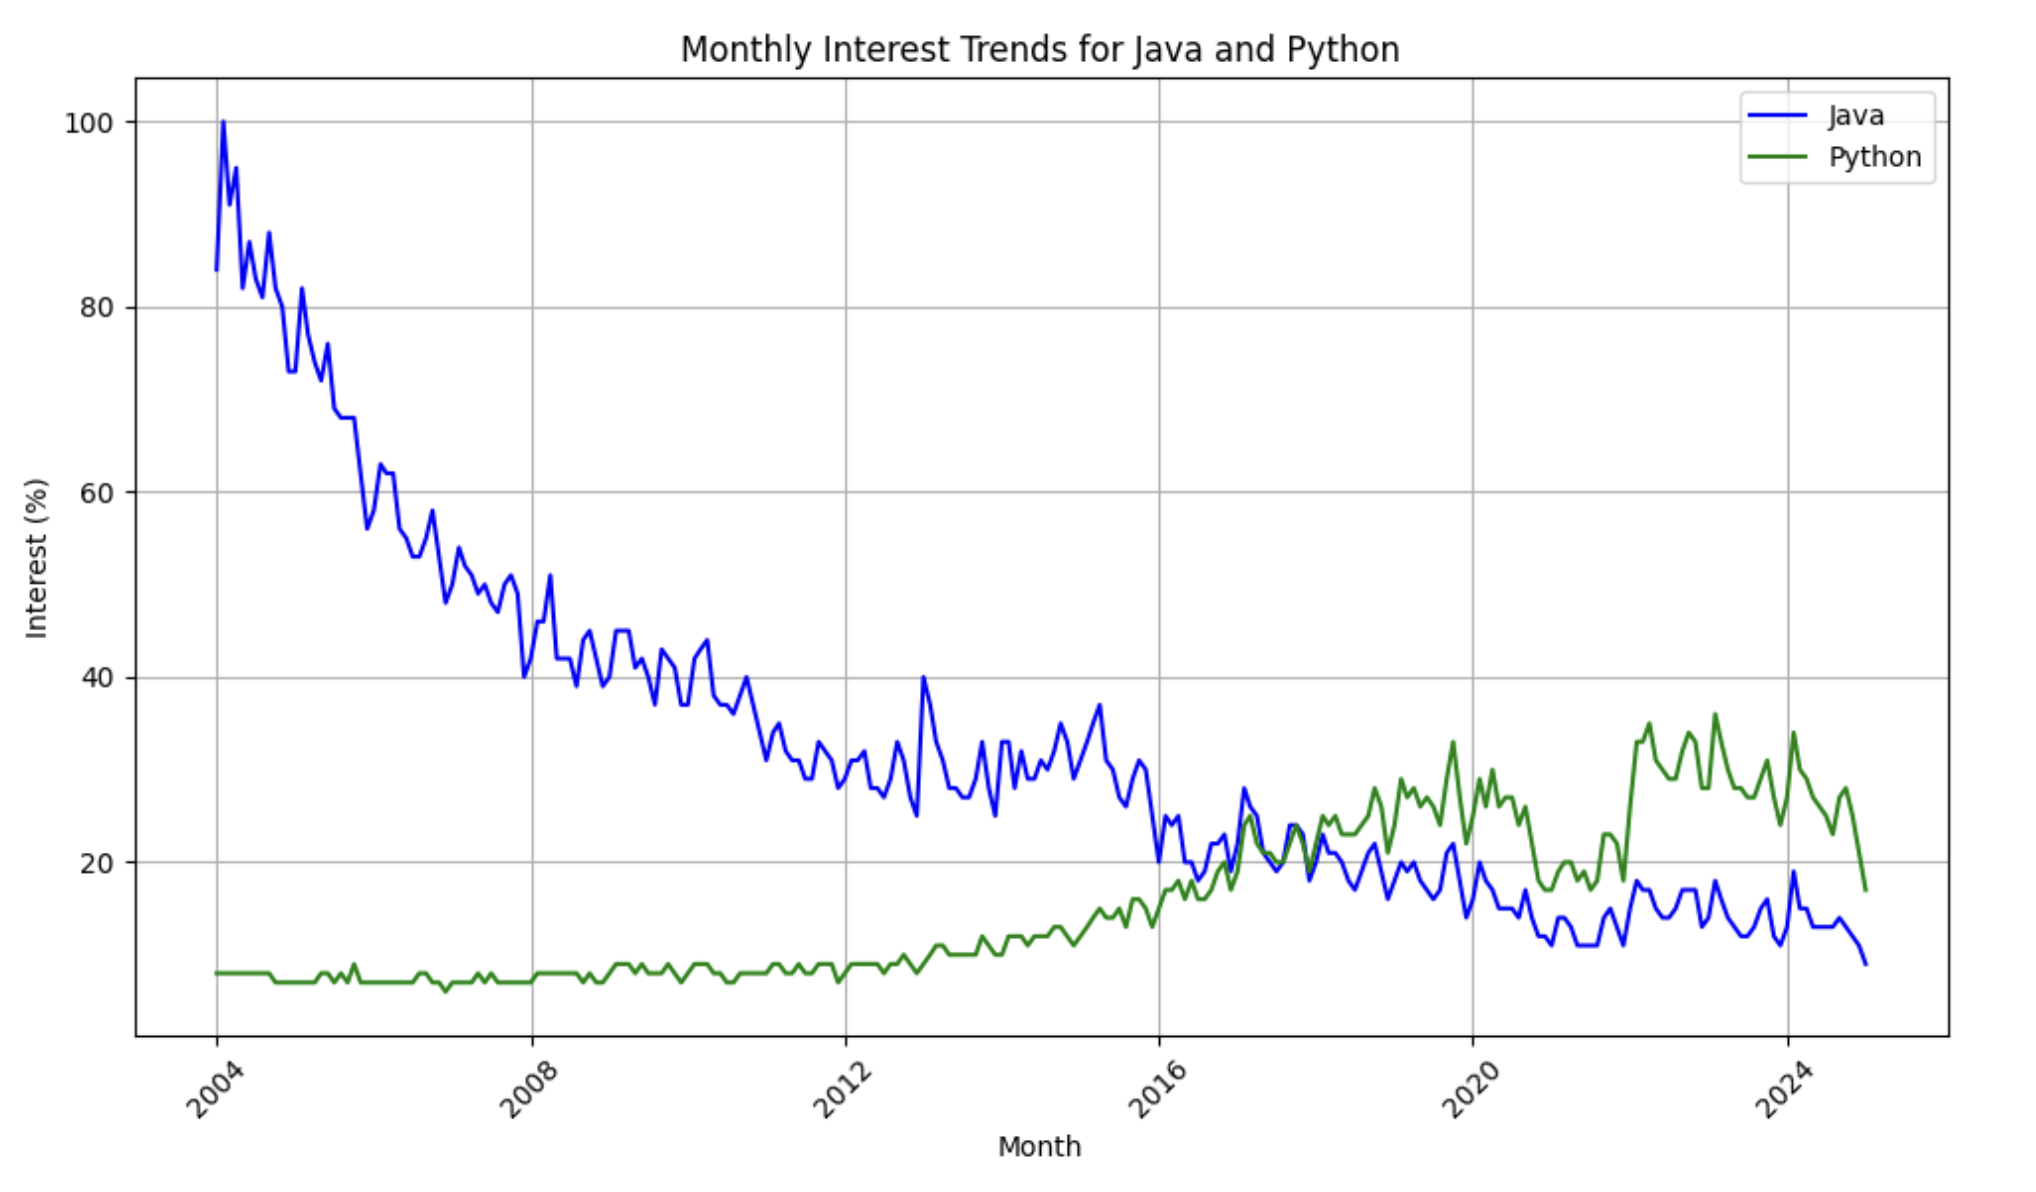
\includegraphics[width=\linewidth]{source/Figure/pythonjavainterest.png}
    \end{center}
    \caption{Java/Python Dominance}
    \label{fig:javapythonadoption}
\end{figure}

Python's dominance can be attributed to functional APIs such as Pandas, Modin, and Dask, a shallow learning curve, and user experience\cite{pererathesis}.  A key benefit of Python is it can interface directly with C/C++ or other native runtimes. Frameworks such as Pandas are not optimized with HPC-compute kernels.  Therefore, bindings such as Cython, which allow access to C++, can be used to create high-performance APIs for high-performance kernels available in HPC clusters such as UVA's Rivanna Supercomputer\cite{shan2022hybrid}.

The rise of Big Data and cloud computing, which began in the early 2000s, played a pivotal role in the emergence of modern artificial intelligence and machine learning. Machine learning and deep learning applications rely heavily on large, predetermined, and preprocessed datasets\cite{abeykoon2020data}. The exponential growth of data has posed significant challenges, particularly in terms of traditional storage and the need for efficient data exchange between distributed storage locations. Cloud computing services, such as Amazon Web Services (AWS), offer innovative solutions to these challenges by providing shared resources, including computing, storage, and analytics\cite{islamBigData}.

Function as a Service (FaaS) is a rapidly evolving paradigm in cloud computing applications. In FaaS, users focus on writing code that is broken down into individual functions. This approach allows users to concentrate on the application code itself, rather than the deployment and management of the underlying compute and storage infrastructure. Serverless functions also offer elasticity and fine-grained billing capabilities. However, serverless does not currently support efficient communication in the form of message passing for large-scale parallel data processing applications, such as Cylon\cite{copik2023fmi}. To address this limitation, Network Address Translation (NAT) in the form of TCP Hole Punching presents a high-performance and cost-effective alternative to other approaches, such as object or in-memory storage\cite{moyer2021punching}.

In this paper, we’ll delve into the concept of Cylon, a runtime engine designed to optimize the execution of deep learning applications in both high-performance computing (HPC) and cloud environments. We’ll explore the advantages of executing workloads within Docker containers on AWS using ECS tasks or managed Docker, and discuss how this approach can be extended to HPC environments utilizing Singularity or Apptainer.

We’ll then demonstrate the seamless integration of Docker execution environments with bare metal servers, showcasing that the runtime semantics are remarkably similar to those of native Docker containers, with minimal performance trade-offs.

Next, we’ll address the challenges associated with large-scale parallel execution on AWS and present the FMI library as a proof of concept for executing Cylon preprocessing and inference on FaaS environments. By demonstrating the library’s effectiveness, we’ll highlight its applicability to scientific domains, particularly astronomy.  We'll discuss costs associated with FaaS execution to illustrate the relevance and novelty of this approach compared to serverful execution in traditional HPC environments.

Finally, we’ll emphasize the potential of this work to revolutionize scientific research and data analysis in various fields


\section{Related Works} \label{sec:relatedWorks}

One of the fundamental concepts in data science is the dataframe. In the Python ecosystem, Pandas\cite{mckinney2011pandas} was created as a Python derivative of the R \textit{data.frame} class. However, one significant limitation of Pandas is that it can only execute on a single core. In contrast, frameworks like Apache Spark, a Java Virtual Machine (JVM) framework, offer similar capabilities and improved performance and support the dataframe abstraction. One notable drawback of Spark is that it operates as a framework rather than a standalone Python library. While there is support for Python through PySpark, its usage necessitates the configuration, setup, and deployment of a Spark cluster. The JVM-to-Python translations introduced by Spark add a substantial performance bottleneck compared to the C++-to-Python translation implemented by Cylon and other high-performance Python libraries, which are more lightweight\cite{abeykoon2020data}.

Similar to the Cylon library, the Twister2 toolkit developed by Kamburugamuwe et al. is implemented using the Bulk Synchronous Parallel (BSP) architecture, based on the observed advantages of scalability and performance. It also incorporates a dataframe API implemented in Java\cite{perera2023depth}. A crucial abstraction introduced by Twister2 is TSets, a concept similar to dataframes or equivalently RDDs in Apache Spark or datasets in Apache Flink. Twister2 is regarded as a foundational step towards high-performance data engineering research and serves as a direct precursor to Cylon\cite{pererathesis}.

The Dask, Modin, and Ray Python distributed dataframe packages, built upon the Pandas API, share similar architectural goals with the Cylon architecture.   A related project, Dask-Cudif, provides distribute dataframe capabilities on Nvidia GPUs leveraging both Dask and Pandas to facilitate integration\cite{perera2023depth}.

To address the need for a uniform distributed architecture, Jeff Dean describes Google’s Pathway architecture, which aims to address the future of AI/ML systems as researchers migrate from Single Program Multiple Data (SPMD) to Multiple Program Multiple Data (MPMD). However, this system is closed-source.

In response, the Cylon Radical Pilot has been developed to support the execution of heterogenous workloads on HPCs. \cite{sarker2024radical}

Another related project, Wukong, offers a similar capability including support for AI/ML inference but was built on serverless FaaS, where AWS handles provisioning, scaling, and other undifferentiated activities. This DAG execution framework has demonstrated near-ideal scalability by executing jobs approximately 68 times faster while achieving close to 92 percent cost savings compared to NumPyWren. \cite{carver2020wukong}

A significant challenge in serverless execution, particularly for parallel data processing applications, is data transfer between running functions. Moyer proposes a solution that leverages Nat Traversal via TCP Hole Punching through an external rendezvous server to enable direct TCP connections between a pair of functions. For an experiment involving over a hundred functions, this approach resulted in a performance improvement of 4.7 times compared to using object storage. \cite{moyer2021punching}

A notable difference between Moyer’s work and the FMI library lies in Moyer’s implementation, which utilizes web sockets for communication. In contrast, FMI is developed as a C++ library similar to the Cylon runtime, making it highly applicable to runtime parallel processing tasks on serverless architectures. 




\section{Preparation Plan}
\label{sec:plan}

\begin{itemize}

\item Jan 23: Cylon on AWS Proposal and initial formulation of Qualification committee.  Began work on UCC/UCX 
\item March 23: Presented Cylon and AWS Work to Professor Yue Cheng's Data science 5110 class during a lecture
\item April 23: Received funding attached to NSF grant to use AWS. Applied for AWS Research grant
\item September 23: Applied UCC/UCX work to bare metal Rivanna to conduct derivative experiments
\item October 23: Received 30k grant from AWS
\item June 23: Successfully executed Cylon experiments on AWS Fargate
\item September 23: Began work integrating NAT Traversal in UCX/UCC
\item February 24: Presented Cylon and AWS Work to Professor Judy Fox's Data science 5110 class during a lecture
\item May 24:  Based on challenges and hurdles implementing Nat Traversal (TCP Hole Punching) in the UCX TCP transport, pivoted to recreating the FMI library as a custom AWS Lambda runtime for future integration into Cylon as a communicator.  This validated the NAT Holepunching capability as a viable option for high-performance communication in AWS Lambda.
\item June 24: Presented Serverless Cylon architecture and subset of work during WOSCx3 Serverless Computing Conference
\item September 24: Built Cylon UCC/UCX Singularity container, allowing derivative experiments across HPC and Clouds.  Developed Qualification exam abstract.
\item October 24: Reran experiments reconfigured for Lambda experiments and also to address error rates.  Discovered changes to the AWS Fargate stack that prevented executing of Cylon using UCX.  This third round of experiments excluded AWS Fargate for this reason.
\item December 24: Contributed FMI work for the Cloud-based Astronomy Framework (CAI).  Demonstrated the use of FMI and the use of AWS Lambda as a critical impact of cost.  Detailed experiments using collective operations to provide summation across multiple running lambda function.
\item January 25: Completed draft for Qualification Report Paper and developed proposal presentation
\item February 25: Qualification Exam Proposal
\end{itemize}

\section{Design and Implementation}
\label{sec:design}

This section outlines the overarching design of Cylon. The design is shaped by insights gained from developing the Twister2 toolset. Specifically, Cylon aims to achieve the following goals: 1) High performance and scalability, 2) An extensible architecture, 3) User-friendly APIs, and 4) Integration across multiple platforms. Following this overview, we will shift to an analysis of our AWS stack's semantics, which builds on this groundwork. We will explore the challenges and architecture of serverless data engineering at scale, emphasizing the novelty and importance of our work\cite{pererathesis}.

\subsection{Cylon Design}

We have developed Cylon to address shortcomings, interact directly with high-performance kernels, and perform better than libraries such as Pandas.  Cylon represents an architecture where performance-critical operations are moved to a highly optimized library. Moreover, the architecture can leverage the performance associated with in-memory data and distributed operations and data across processes, an essential requirement for processing large data engineering workloads at scale. Such benefits are realized, for example, in the conversion from tabular or table format to tensor format required for Machine Learning/Deep Learning or via relational algebraic expressions such as joins, select, project, etc. A key aspect of the Cylon architecture is the intersection of data engineering and AI/ML, allowing it to interact seamlessly with frameworks such as Pytorch\cite{pytorch2019} and TensorFlow\cite{tensorflow2015}.

\begin{figure}[H]
    \centering
    \includesvg[width=\linewidth]{Figure/cylon_arch}
    \caption{Cylon Architecture}
    \label{fig:cylonarch}
\end{figure}

Figure \ref{fig:cylonarch} offers a high-level overview of the Cylon Architecture. Solid boxes denote features and capabilities implemented within the Cylon runtime. The table layer encompasses tables, arrays, and scalars managed by the Apache Arrow runtime. The communication layer represents the interface between Cylon and supported communication libraries. Currently, Cylon supports OpenMPI, UCX, and Gloo. Both distributed and local operators are supported. Cython bindings facilitate Python access to C++ data structures, functions, and classes.

\begin{figure}[H]
    \centering
    \includesvg[width=\linewidth]{Figure/cylon_comm_arch}
    \caption{Cylon Communication Model}
    \label{fig:cyloncomm}
\end{figure}

Figure \ref{fig:cyloncomm} illustrates the Cylon communication interface. Two key features of this model are its modular architecture and extensibility, as discussed in \cite{pererathesis}. To simplify the complexities of distributed programming, frameworks like TCP and Infiniband facilitate plug-and-play configuration, supporting high-performance communication libraries such as OpenMPI, UCX, and Gloo. The Cylon architecture is based on the Apache Arrow Columnar format. This library offers serialization-free copying across various runtimes, including Pandas and Numpy, as mentioned in \cite{pererathesis}. We anticipate that Cylon will profoundly impact the development of high-performance data engineering frameworks and ultimately contribute and help shape the integration of ML/AI pipelines. 

\subsection{Pillars of Cloud Computing and Well-Architected Cloud Systems}
Cloud computing is widely regarded as the cornerstone of the fourth industrial revolution. As companies and organizations increasingly rely on Big Data and Artificial Intelligence, cloud providers like AWS are pivotal in facilitating integration and innovation to support these endeavors. \cite{hashemipour2020amazon} AWS offers four fundamental pillars for successful cloud architectures. First, cloud architectures eliminate the uncertainty surrounding capacity requirements. Second, they provide virtually unlimited usage, enabling architectures to scale up and down autonomously. Third, cloud architectures facilitate testing systems at production scale. In other words, production-like environments can be created on demand.
Furthermore, these environments can simulate production environment conditions or internet-scale conditions at significantly lower costs compared to on-premise architecture. Cloud architectures also lower the risk associated with architectural change by removing the test serialization problem with on-premise infrastructure.  This refers to the situation that can occur with software testing on-premise.  In this case, tests are often executed in parallel due to limitations with shared resources or hardware constraints.  This can slow testing and create other bottlenecks that complicate testing and evaluation.  To address this problem, cloud systems support automation as an enabler of architectural experimentation. This allows for the creation and replication of systems at low costs and enables tracking and auditing of impact with low effort.  Lastly, cloud architectures allow for evolutionary architectures.  This includes automating and testing on-demand to lower the impact of design change.  With evolutionary architectures, systems can evolve over time so that it is possible to take advantage of innovation(s) as standard practice\cite{aws_well_architected_framework}.

Well-architected cloud systems are built on four key pillars: security, reliability, performance efficiency, and cost optimization\cite{aws_well_architected_framework}.

Security protects information systems and assets while delivering value through risk assessment and mitigation strategies. It involves applying security at all layers, enabling traceability, automating responses to security events, and treating automation as a best practice\cite{aws_well_architected_framework}.

Reliability refers to a system’s ability to recover from infrastructure or service failures, acquire resources dynamically to meet demand, and mitigate disruptions such as misconfiguration or transient network issues. Design principles of reliability include testing recovery procedures, automating recovery from failures, using horizontal scalability to increase aggregate system availability, and eliminating guesswork about capacity\cite{aws_well_architected_framework}.

Performance Efficiency denotes the ability to use computing resources efficiently to meet system requirements and maintain that efficiency as demand changes and technology evolves. Key principles related to performance efficiency include democratizing advanced technologies, going global in minutes, and experimenting often\cite{aws_well_architected_framework}.

Cost Optimization involves avoiding unnecessary costs and suboptimal resource use. Effective cost optimization includes using managed services to reduce the overall cost of ownership, trading capital expenses for operating expenses, taking benefits from economies of scale, and reducing spending on data center operations\cite{aws_well_architected_framework}.

This paper's serverless and serverful work aligns with the best practices outlined in the discussed pillars of successful cloud architectures and the key characteristics of well-architected cloud architectures. The author has also successfully built and designed well-architected cloud software. Notably, he was pivotal in integrating SiriusXM/Pandora streaming APIs with the Amazon Alexa infrastructure. This infrastructure operates at internet scale and processes millions of requests daily for streaming content and metadata.

\subsection{Implementation}
As part of this work, We have implemented high-performance data engineering on serverful and serverless environments using the Cylon and FMI libraries.  We will discuss each implementation in detail and outline our plan and the current effort to integrate the FMI library into Cylon as a communicator.

\subsection{Cylon High Performance Communication}
Data parallelism in Cylon is built around Bulk Synchronous Parallel (BSP), a model that uses Single Program Multiple Data (SPMD) across compute nodes.  The Message Passing Interface (MPI) is implemented by frameworks such as OpenMPI, MPICH, MSMPI, IBM Spectrum MPI, etc.

For most use cases, parallel data processing with OpenMPI Cylon is standard, based on the OpenMPI library’s availability on HPCs like Rivanna and Summit. However, MPI isn’t compatible with all frameworks, such as Dask and Ray. These distributed libraries are better suited for cloud technologies like Kubernetes and Amazon Elastic Container Service (ECS). OpenMPI includes process bootstrapping capabilities that facilitate the initialization of communication primitives and configuration. Cloud environments like AWS don't require this process management capability; therefore, communication libraries such as UCX/UCC are ideal.  Another benefit associated with UCX is the library is designed to be decoupled from network hardware.  This provides increased portability while ensuring high performance and scalability.  A key benefit of UCX is that it allows access to GPU memory and bidirectional GPU communication.  This library also supports Remote Direct Memory Access (RDMA) over Infiniband and Converged Ethernet (ROcE).  Additionally, zero-copy GPU memory copy over RDMA is supported, leading to exceptional performance.  OpenSHEM is also included to support parallel programming\cite{shan2022hybrid}.

For Cylon and as part of this work, we implemented a configuration mechanism that is modularized in such a way as to enable the implementation of new sources as they become available. We use Redis as a key-value store for our experiments to facilitate the bootstrapping process and provide barrier conditions.
Another interesting detail about our implementation concerns resource usage, specifically with Unified Communication Protocols (UCP) or endpoints for a network connection.  UCC also uses endpoints for collective operations. Unfortunately, reusing endpoints is impossible; therefore, we implemented separate endpoints for both UCC and UCP. This feature is not included with UCC/UCX and is necessary for parallel pre-processing tasks and BSP style execution using Cylon. The integration of UCX as a Cylon communicator involves the following: 1) Serializer, 2) Communication Operators, 3) Channels and AllToAll, and 4) Integration with dataframe operators\cite{shan2022hybrid}.  

Within Cylon, the UCX communicator serializes tables, columns, and scalars into buffers before being passed to the network communication layer.  As was mentioned earlier, Cylon implements a Distributed Memory Dataframe (DDMF) via Apache Arrow. This is represented as a collection of \textit{P} dataframes or partitions of lengths $\{ N_0,...N_{P-1}\}$ and a schema denoted as $S_m$.  The total length of the Distributed Memory Dataframe can be represented as $\sum{N_i}$ and the concatenation of row labels as $R_n=\{R_0, R_1, ... R_{P-1}  \}$.  Figure \ref{fig:distdataframe} illustrates this process.

\begin{figure}[ht]
    \begin{center}
    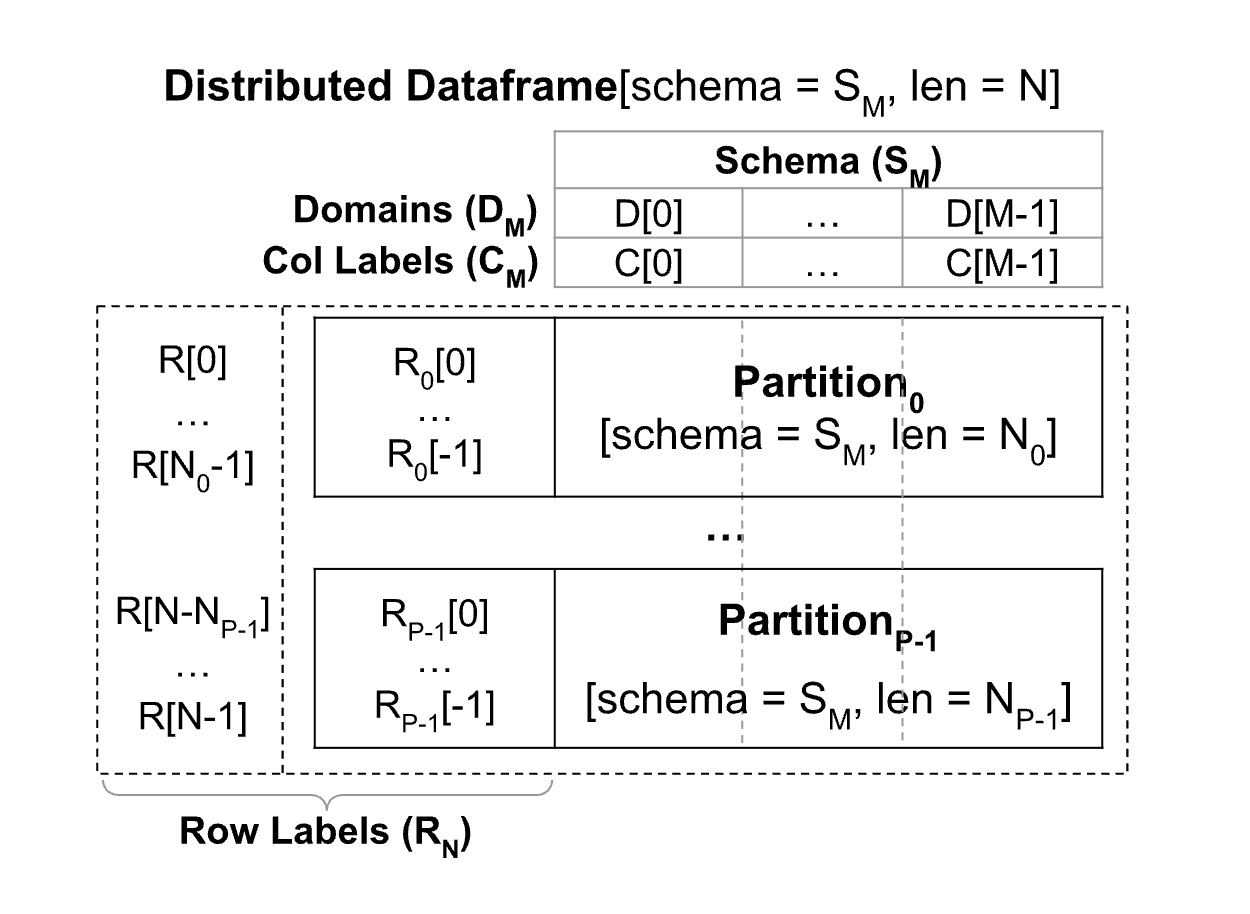
\includegraphics[width=\linewidth]{source/Figure/distDataframe.png}
    \end{center}
    \caption{Distributed Memory Dataframe (DDMF)\cite{pererathesis}}
    \label{fig:distdataframe}
\end{figure}

The Cylon channels API implements the AllToAll operation as point-to-point communication and uses the UCC library for  collective operations such as AllGather.  Distributed operators are implemented generically within Cylon.  The experiments detailed in the next section use the Distributed Join DataFrame operator.  For this case, the process follows: 1) Hash applicable columns into partitioned tables, 2) Use AllToAll to send tables to the intended destination, and 3) Execute a local join on the received tables\cite{shan2022hybrid}.

The initialization or bootstrapping of the Cylon UCX/UCC communicator necessitates the provision of communication metadata during startup. This metadata includes each process's world size, rank, and endpoint address. We utilize the \textit{Redis} key-value store to facilitate this exchange. Our design increments an atomic value to represent the rank. Before incrementing the value, the rank is set. Redis is launched externally to the Cylon processes. The only requirement is that the \textit{Redis} host be provided before initializing the Cylon runtime. Our experiments employed a combination of AWS ElastiCache, Redis, and ECS tasks that include the dockerized \textit{Redis} runtime. Depending on the specific experiment’s communication requirements, we selected a combination of \textit{Redis} deployments. One implementation limitation is that the stored metadata on \textit{Redis} must be cleared between subsequent experiments. Otherwise, the experiment executes non-deterministically and ultimately fails. In the case of executing N experiments of a given class (e.g., world size of 8 for 9.1 million rows), we need to configure N \textit{Redis} hosts when running experiments in parallel.

\begin{figure}[ht]
    \begin{center}
    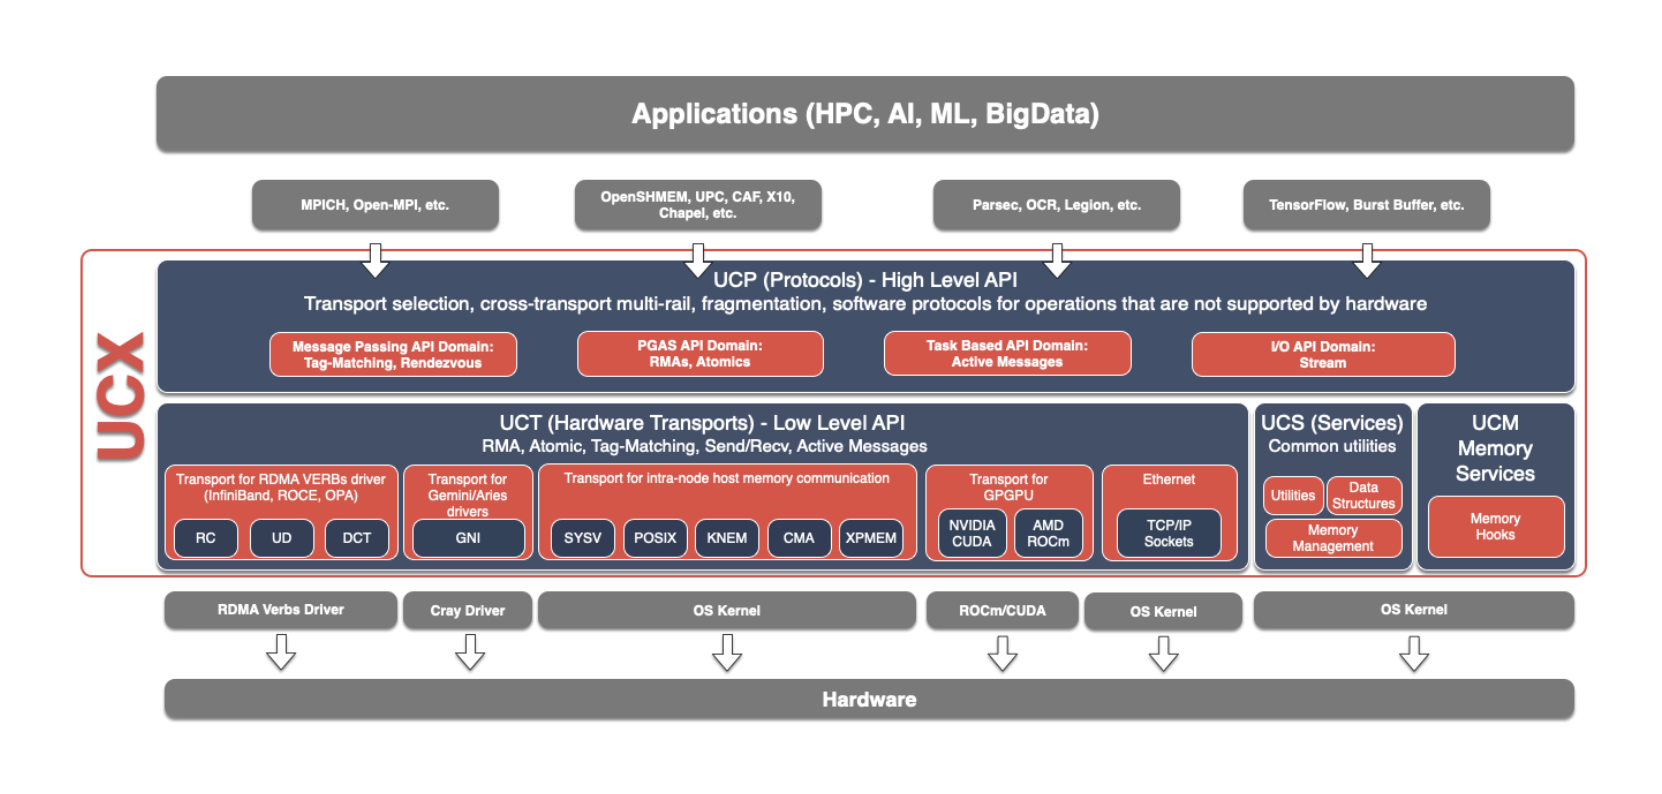
\includegraphics[width=\linewidth, height=200pt]{source/Figure/ucxarchitecture.png}
    \end{center}
    \caption{Unified Communication X (UCX) Library Architecture\cite{shamis2015ucx}}
    \label{fig:ucxarch}
\end{figure}

Our experiment design, which utilized UCX/UCC, proved highly effective for most AWS and HPC experiments. One aspect of our design involved using Docker. This product uses OS-level virtualization to deploy software in packages or containers to create a runtime environment that could be seamlessly deployed across both HPC and AWS\cite{dockerwiki}. We pushed our Dockerized environments to Dockerhub and employed Apptainer on Rivanna to construct a Singularity container encapsulating the Cylon runtime. A significant advantage of this approach is that modifications to the environment (or Dockerfile) were not required. Consequently, all our experiments utilized the same runtime, resulting in a consistent and derivative approach across infrastructure.  We believe our architecture and the inclusion of UCX/UCC to be a novel contribution, and based on our research, it is the only case we could find where UCC/UCX was being used for ML/AI pipelines such as Cylon.

A crucial aspect of this research involves executing data engineering pre-processing on serverless compute. For this subset of our study, we made a minor modification to the UCX Unified Communication Transport (UCT) lower-level API. This change was necessary due to UCX’s initialization behavior. UCX employs low-level system calls to select the most suitable and optimal communication protocol based on the available resources. However, only TCP is supported for serverless computing. We observed that the UCX device query incorrectly retrieved the incorrect IP address from the hardware during initialization. To ensure successful initialization, we had to override the IP address discovered by UCX. This modification enabled us to conduct experiments on AWS Fargate, a serverless Docker running on ECS, a fully managed container orchestration service. Unfortunately, this capability was deprecated due to changes in the underlying serverless architecture implemented by AWS.  This led us to investigate other potential communication options for BSP systems that run on serverless systems.

A similar issue was encountered with AWS Lambda functions, a serverless compute service or Function as a Service (FaaS) that allows code to execute in response to events and automatically manages and scales resources. We could not leverage the IP address override capability mentioned above to execute Cylon on AWS Lambda due to the unavailability of system calls similar to AWS Fargate. One solution presented by Copik et al. was to use NAT traversal or TCP hole punching to enable direct communication between a pair of AWS Lambda functions via the FMI library. Unlike storage-based solutions, direct communication increases communication time by multiple orders of magnitude.  Figure \ref{fig:natholepunching} illustrates this process.  NAT hole punching requires functions to be behind a NAT gateway.  The gateway hides the addresses of each function by rewriting the internal addresses with an external address.  Outgoing communication creates an entry in the translation table.  This results in replies being sent to the intended recipient.  The NAT Gateway will drop packets routed to addresses not found in the translation table.  In order to support NAT hole-punching, a publicly accessible server is required that creates entries in the translation table and relays addresses between two functions.  


\begin{figure}[ht]
    \begin{center}
    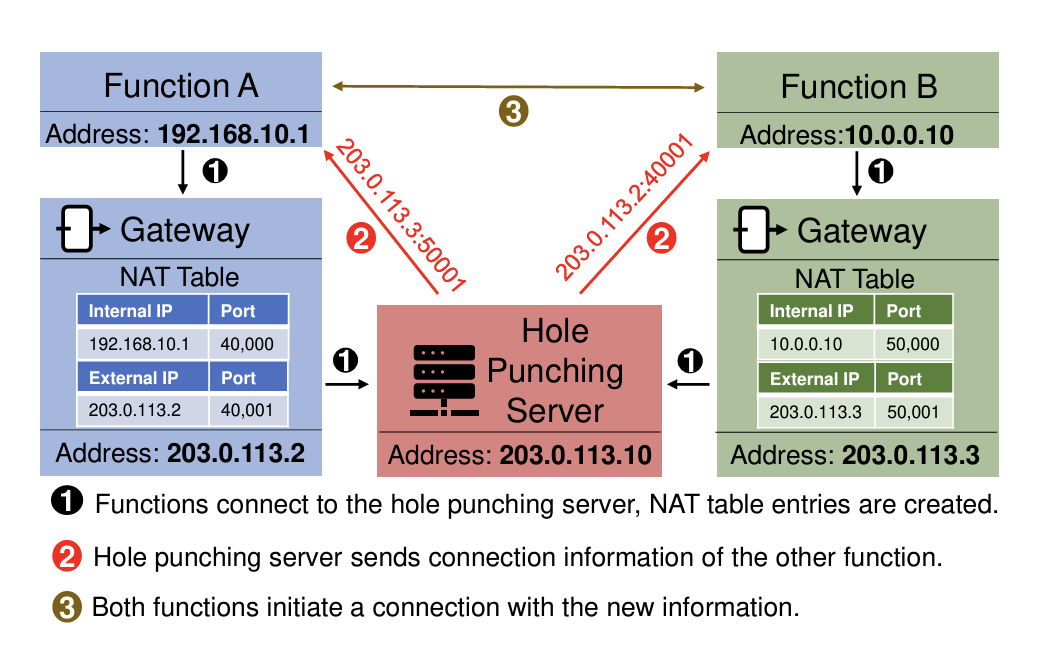
\includegraphics[width=\linewidth]{source/Figure/NatHolePunching.png}
    \end{center}
    \caption{Network Address Translation (NAT) Hole Punching\cite{copik2023fmi}}
    \label{fig:natholepunching}
\end{figure}

We created an ECS or Docker image with a C++ implementation of a relay or rendezvous server for our experiments.  Our initial goal was to integrate the FMI library into Cylon as a modification of the existing TCP UCT UCX source.  Unfortunately, this approach yielded unsuccessful results based on the UCX TCP architecture and NAT hole-punching address exchange semantics.  We believe an ideal approach is implementing FMI as a separate Cylon communicator, similar to the UCC/UCX communicator described above.  We successfully recreated and validated the FMI library's capability as a custom AWS Python Lambda Docker image.   For this work, we created a Dockerfile with all the libraries necessary for experiment execution.  We also implemented the AWS Lambda interface and created derivative experiments like the distributed join experiments detailed in the next section.  Including this library is an ideal choice based on the limitations imposed by AWS Lambda and the fact that a higher-level abstraction is necessary for direct communication between Lambda functions.  There are also cost considerations based on the AWS Lambda cost model, where request rate, execution time, and function size correlate to the overall cost.  Direct communication leads to optimized usage of Lambda functions and allows full usage of the available provisioned CPU and memory.

\begin{figure}[ht]
    \begin{center}
    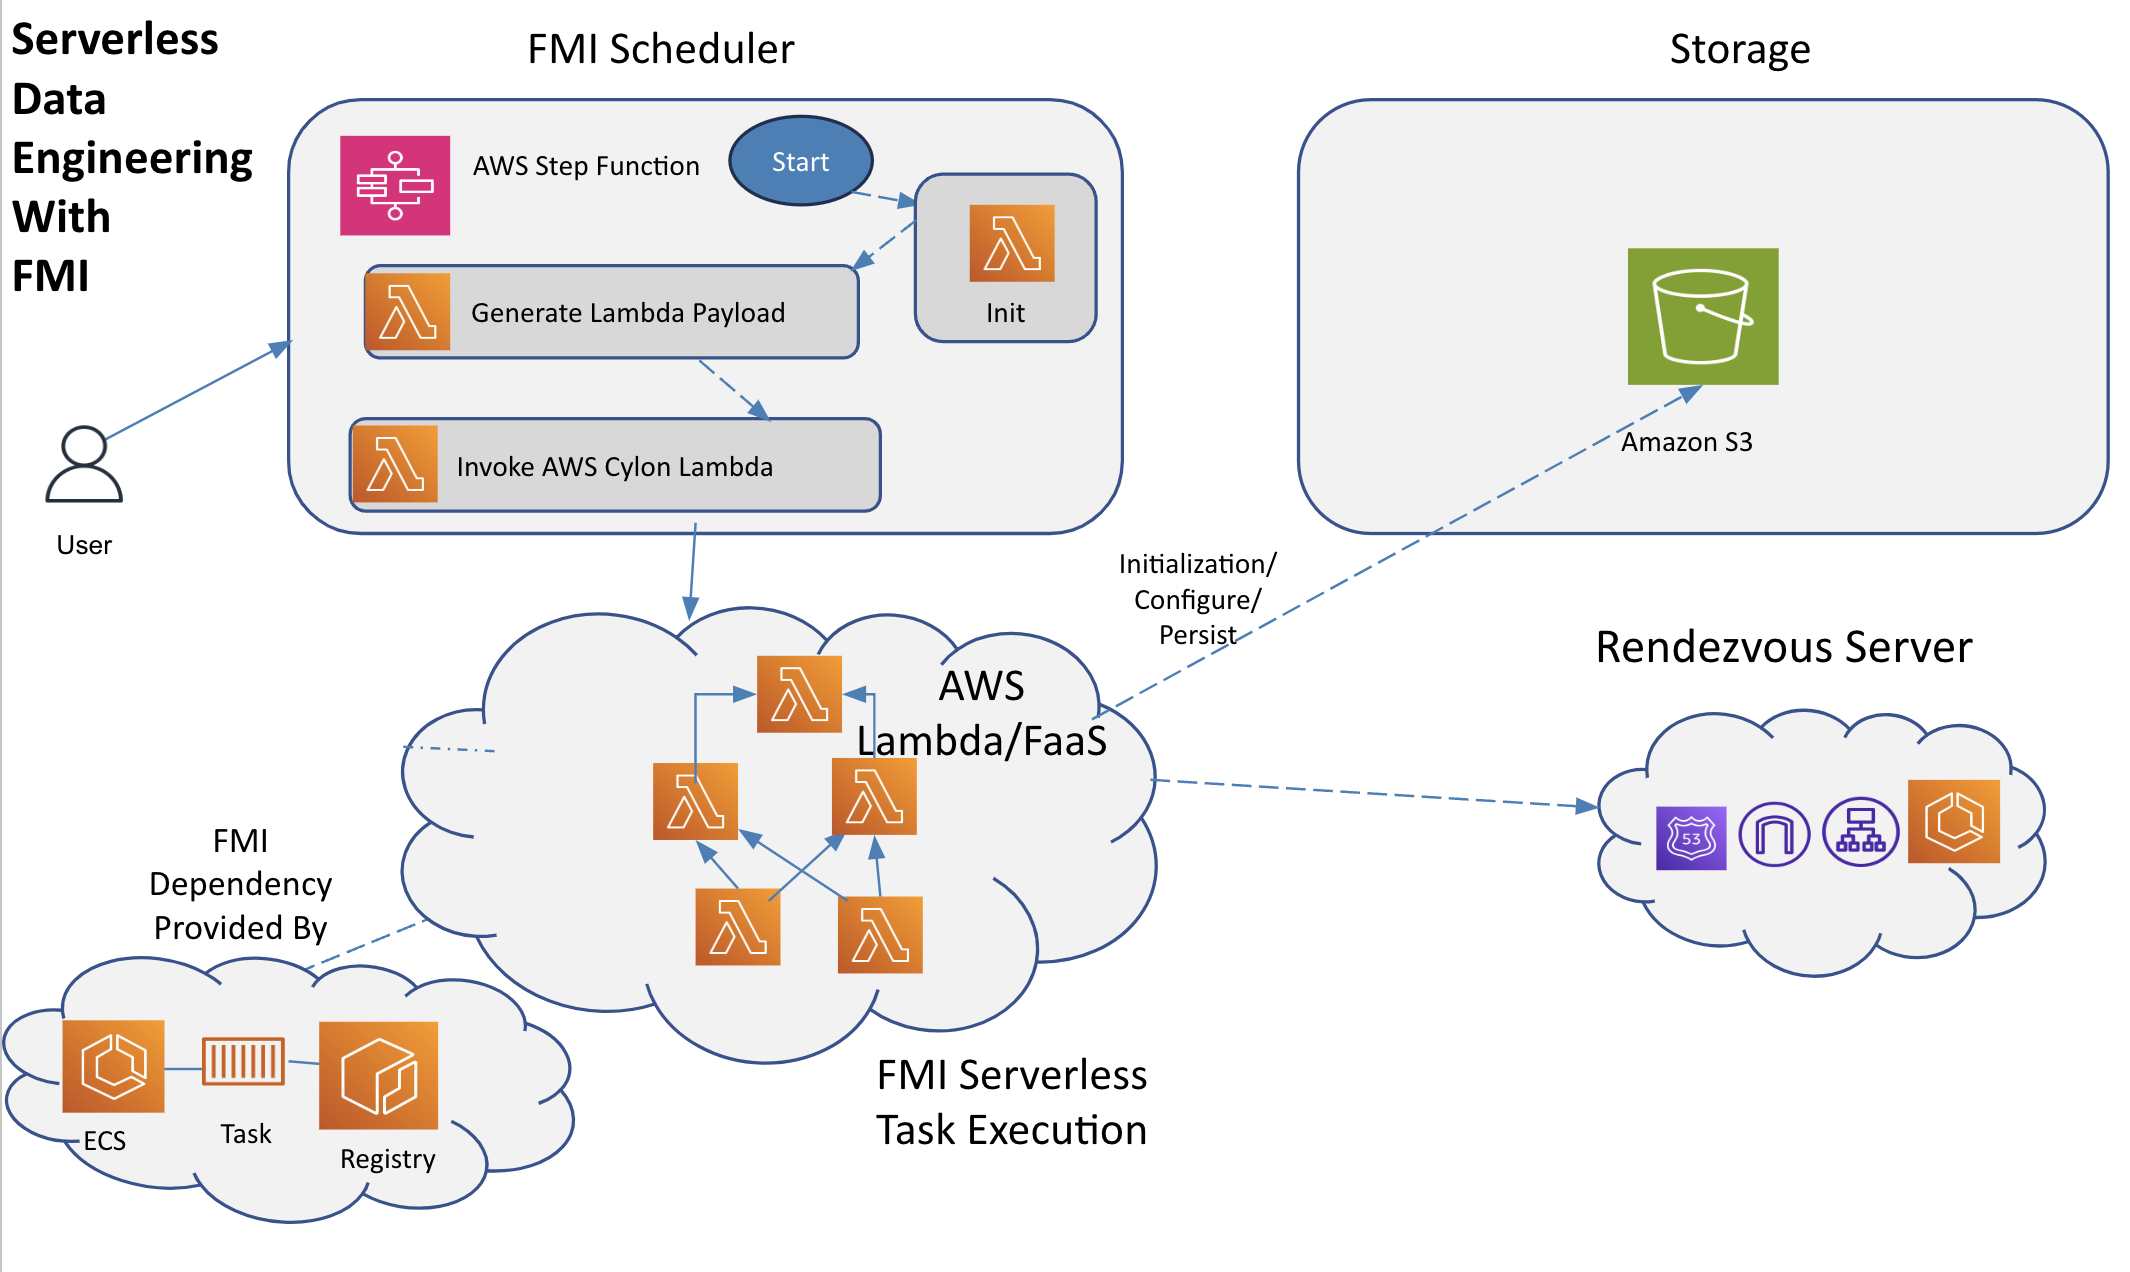
\includegraphics[width=\linewidth]{source/Figure/serverlessdataengineering.png}
    \end{center}
    \caption{Serverless Data Engineering Architecture}
    \label{fig:serverlessdataengineering}
\end{figure}

Figure \ref{fig:serverlessdataengineering} illustrates our architecture. To implement the FMI scheduler, we created an AWS Step Function, as depicted in Figure \ref{fig:fmistatemachine}. AWS Step Functions are a Software as a Service (SaaS) feature that facilitates the orchestration of AWS services into serverless workflows. The \textit{Lambda: init} start function receives a payload containing various parameters, such as the number of rows, world size, number of iterations, target S3 bucket, script, and output paths. We utilize a specific S3 bucket and push the invocation results to a folder using the \textit{Boto3} library. This approach is advantageous over parsing the data output from log files in AWS CloudWatch, a SaaS metrics repository created and utilized by AWS services, as it would be cumbersome. The Lambda init function sends the input JSON payload to the \textit{fmi\_init} AWS Lambda function. This function validates the rendezvous server’s availability and generates an N-sized array of JSON payloads, which are then sent to the \textit{Map}, \textit{ExtractAndInvokeLambda} states. The \textit{Map} state includes inline and distributed processing modes.   We choose the Distributed processing mode to enable highly parallel execution. Next, each generated payload is sent to the Lambda: Invoke state from the pass \textit{ExtractAndInvokeLambda} state.  This state passes the input to output, which executes the \textit{fmi\_executor} AWS Lambda function. The runtime of the \textit{fmi\_executor} function includes the runtime described earlier, which includes the FMI library. The incoming payload specifies the location of the target script in the S3 bucket. Upon execution of the Lambda function, the contents of the specified S3 bucket are retrieved and persisted into temporary ephemeral storage. Subsequently, Python3 executes the script used for our experiments (i.e., scaling.py). We support a single script and a folder containing Python scripts and modules. For our experiments, we combined FMI and Cylon experiments in our scaling.py Python script to facilitate execution across serverless, serverful, and HPC environments\cite{cloudmeshcommon}. 



\begin{figure}[ht]
    \begin{center}
    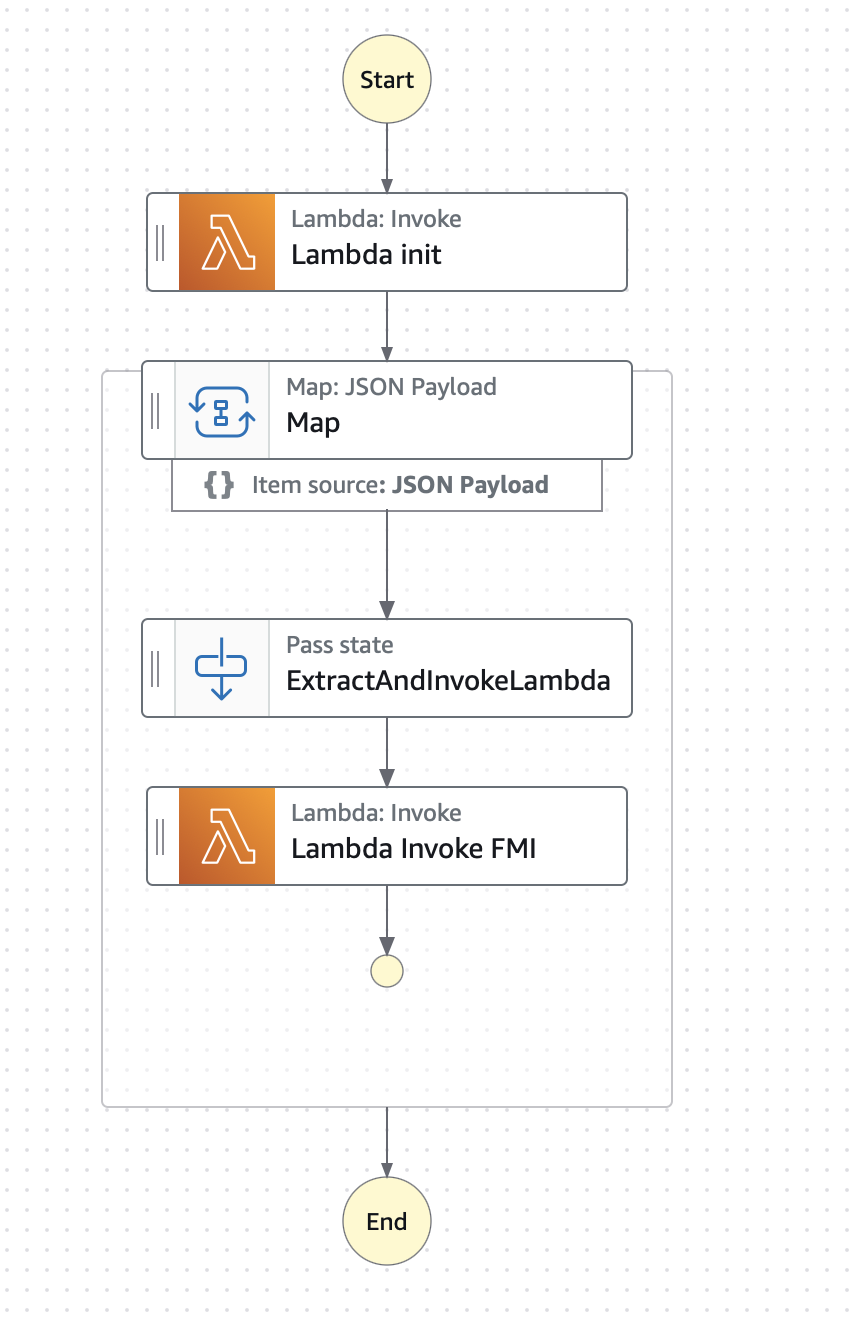
\includegraphics[width=\linewidth]{source/Figure/FMIStateMachine.png}
    \end{center}
    \caption{AWS Step Function for Serverless Data Parallel Task}
    \label{fig:fmistatemachine}
\end{figure}


During execution, the \textit{fmi\_executor} connects with the Rendezvous Server referenced in Figure \ref{fig:serverlessdataengineering}.  Once the second function in the pair connects to the Rendezvous Server, both servers receive the destination function's public address.  The Python script then continues to execute until the collective operation is performed.  For the experiments discussed below, we use an AllReduce collective to calculate a summation of start-to-end execution across the world size of executing functions.  We also use the cloudmesh stopwatch library to facilitate logging and benchmarking the runtime of our executing experiments.
\section{Experiments}

We conducted three sets of experiments detailed by Table \Ref{tab:exp_table1}, Table \Ref{tab:exp_table2}, and Table \Ref{tab:exp_table3}.  For the first set of experiments, we used a calculation to determine the number of rows for both weak and strong scaling.  First, we calculated data per core as memory per code divided by workspace allocation (both four based on previous Summit HPC experiments).  Next, we calculate data per table as data per core divided by three for weak scaling and memory per node divided by workspace allocation multiplied by the number of tables used for a join.  The number of rows for weak scaling was calculated as data per table divided by bytes per row multiplied by $10^9$.  We use a defined row size of 800,000 for the second set of experiments and a very small instance/configure size based on memory availability on AWS T2 instances as the lowest common denominator.  The third set of experiments was configured based on memory available to AWS Lambda functions which is 10240 MB maximum.  Therefore, we configured a max and close to half-size configuration for each set of experiments to be 10MB and 6MB.  

\begin{table}[!hbp]
    \centering
    \small
   \captionsetup{justification=centering}
    \caption{Experiments Setup on UVA Rivanna HPC and Amazon Web Services. WS/SS = weak/strong 
         scaling; M=Million}
        \begin{tabular}{|>{\centering\arraybackslash}p{2.2cm}|>{\centering\arraybackslash}p{2.8cm}|>{\centering\arraybackslash}p{2cm}|} % Added vertical lines on both sides
        \hline
        \textbf{Experiment Description} & \textbf{Rows} & \textbf{Rows Size} \\
        \hline
        AWS ECS EC2 8 CPU/26 GB Mem WS/SS & 1-32 & [9.1 | 145M]  \\
        \hline
        AWS ECS EC2 16 CPU/28 GB Mem WS/SS & 1-32 & [9.1 | 145M]  \\
        \hline
        AWS ECS Fargate 8 CPU/26 GB Mem WS/SS & 1-32 & [9.1 | 145M]  \\
        \hline
        AWS ECS Fargate 16 CPU/28 GB Mem WS/SS & 1-32 & [9.1 | 145M]  \\
        \hline
        Rivanna 8 CPU WS/SS & 1-32 & [9.1 | 145M]  \\
        \hline
        Rivanna 16 CPU WS/SS & 1-32 & [9.1 | 145M]  \\
        \hline
    \end{tabular}
    \label{tab:exp_table1}
\end{table}

\begin{table}[!hbp]
    \centering
    \small
   \captionsetup{justification=centering}
    \caption{Experiments Setup on UVA Rivanna HPC and Amazon Web Services to measure raw performance of CPUs. WS = weak/strong 
         scaling; M=Million}
        \begin{tabular}{|>{\centering\arraybackslash}p{2.2cm}|>{\centering\arraybackslash}p{2.8cm}|>{\centering\arraybackslash}p{2cm}|} % Added vertical lines on both sides
        \hline
        \textbf{Experiment Description} & \textbf{Rows} & \textbf{Rows Size} \\
        \hline
        EC2 Nano (1 vCPU, 1 core) WS & 1 & 800000  \\
        \hline
        EC2 Micro (1 vCPU, 1 core) WS & 1 & 800000  \\
        \hline
        Fargate .25 CPU 1 core WS & 1 & 800000  \\
        \hline
        Fargate .50 CPU 1 core WS & 1 & 800000  \\
        \hline
        Rivanna Standard (1 Node, 1 Thread, 1 CPU, 1 Core) WS & 1 & 800000  \\
        
        \hline
    \end{tabular}
    \label{tab:exp_table2}
\end{table}

\begin{table}[!hbp]
    \centering
    \small
   \captionsetup{justification=centering}
    \caption{Experiments Setup for Comparative to AWS Lambda on UVA Rivanna HPC and Amazon Web Services. WS/SS = weak/strong 
         scaling; M=Million}
        \begin{tabular}{|>{\centering\arraybackslash}p{2.2cm}|>{\centering\arraybackslash}p{2.8cm}|>{\centering\arraybackslash}p{2cm}|} % Added vertical lines on both sides
        \hline
        \textbf{Experiment Description} & \textbf{Rows} & \textbf{Rows Size} \\
        \hline
        AWS ECS EC2 4 CPU/15 GB Mem WS/SS & 1-64 & [9.1 | 4.5M]  \\
        \hline
        AWS ECS EC2 2 CPU/7.5 GB Mem WS/SS & 1-64 & [9.1 | 4.5M]  \\
        \hline
        \hline
        Rivanna 10 GB Mem WS/SS & 1-64 & [9.1 | 4.5M]  \\
        \hline
        Rivanna 6 GB Mem WS/SS & 1-64 & [9.1 | 4.5M]  \\
        \hline
        Lambda 10 GB Mem WS/SS & 1-64 & [9.1 | 4.5M]  \\
        \hline
        Lambda 6 GB Mem WS/SS & 1-64 & [9.1 | 4.5M]  \\
        \hline
    \end{tabular}
    \label{tab:exp_table3}
\end{table}

\subsection{Join Operation Scalability}

For the first set of experiments, we measure the average execution time and standard deviation in seconds for the distributed join operation under both weak and strong scaling. We conducted scaling experiments on ECS EC2, Fargate ECS clusters, and Rivanna, the University of Virginia's High-Performance Computing (HPC) cluster for this set of experiments. For Fargate, we employed Ubuntu 22.04.2 LTS (Intel(R) Xeon(R) Platinum 8124M CPU @ 3.00GHz) with a configuration of 16 virtual CPUs and 28 GB of memory, and Ubuntu 22.04.2 LTS (Intel(R) Xeon(R) Platinum 8259CL CPU @ 2.50GHz) configured with four virtual CPUs and 26 GB of memory. For EC2, we used Ubuntu 22.04.2 LTS (Intel(R) Xeon(R) Platinum 8275CL CPU @ 3.00GHz) for hosts configured with up with 16 virtual CPUs and 28 GB of memory, alongside Ubuntu 22.04.2 LTS (Intel(R) Xeon(R) Platinum 8488C) for hosts equipped with four virtual CPUs and 26 GB of memory. We executed derivative experiments for Rivanna on 8 CPU and 16 CPU nodes. Additionally, we conducted four experiments for each node configuration (1, 2, 4, 8, 16). Table \ref{tab:weak-exp_table} summarizes the weak scaling results from join operations for this set of experiments. 


\begin{table}
%\setlength{\tabcolsep}{5pt}
	\centering
	\caption{Execution Time of Weak Scaling from Join Operations Across Infrastructure.}
	\label{tab:weak-exp_table}
	\begin{tabular}{llcr @{\hspace{1\tabcolsep}} lr @{\hspace{1\tabcolsep}} l}
		%
		\toprule
		                   &
		               &
		                     &
		\multicolumn{2}{c}{Execution Time}         \\
	    		%
		Infrastructure             &
		Scaling               &
		Parallelism                     &
		\multicolumn{2}{c}{time (seconds)}                    \\
		%
		\midrule
		\multirow{5}{*}{EC2 8 CPU/26 GB} &
		\multirow{5}{*}{Weak} &
		1                       &
		25.87 & $\pm0.62$     \\
		%
		&
		                     &
		2                     &
		33.82 & $\pm0.42$   \\
		%
		&
		                   &
		4                     &
		34.70 & $\pm0.27$    \\
		%
		                    & &
		8                     &
		34.40 & $\pm0.62$      \\
  		%
		                    & &
		16                     &
		36.04 & $\pm0.35$      \\

        \cmidrule{2-5}
    	\multirow{5}{*}{EC2 16 CPU/28 GB} &
		\multirow{5}{*}{Weak} &
		1                       &
		30.07 & $\pm0.11$     \\
		%
		&
		                     &
		2                     &
		36.75 & $\pm0.51$   \\
		%
		&
		                   &
		4                     &
		36.83 & $\pm0.14$    \\
		%
		                    & &
		8                     &
		37.36 & $\pm0.22$      \\
  		%
		                    & &
		16                     &
		38.40 & $\pm0.37$      \\

		\cmidrule{2-5}
    	\multirow{5}{*}{Fargate 8 CPU/26 GB} &
		\multirow{5}{*}{Weak} &
		1                       &
		33.68 & $\pm0.06$     \\
		%
		&
		                     &
		2                     &
		43.69 & $\pm0.19$   \\
		%
		&
		                   &
		4                     &
		41.93 & $\pm1.03$    \\
		%
		                    & &
		8                     &
		47.86 & $\pm0.63$      \\
  		%
		                    & &
		16                     &
		47.81 & $\pm1.28$      \\
		
		\cmidrule{2-5}
    	\multirow{5}{*}{Fargate 16 CPU/28 GB} &
		\multirow{5}{*}{Weak} &
		1                       &
		33.10 & $\pm0.60$     \\
		%
		&
		                     &
		2                     &
		40.44 & $\pm0.21$   \\
		%
		&
		                   &
		4                     &
		40.98 & $\pm0.09$    \\
		%
		                    & &
		8                     &
		41.65 & $\pm0.07$      \\
  		%
		                    & &
		16                     &
		42.67 & $\pm0.37$      \\

        \cmidrule{2-5}
    	\multirow{5}{*}{Rivanna 8 CPU} &
		\multirow{5}{*}{Weak} &
		1                       &
		18.09 & $\pm0.02$     \\
		%
		&
		                     &
		2                     &
		20.75 & $\pm0.42$   \\
		%
		&
		                   &
		4                     &
		21.29 & $\pm0.68$    \\
		%
		                    & &
		8                     &
		22.17 & $\pm0.33$      \\
  		%
		                    & &
		16                     &
		24.01 & $\pm0.85$      \\
        \cmidrule{2-5}
    	\multirow{5}{*}{Rivanna 16 CPU} &
		\multirow{5}{*}{Weak} &
		1                       &
		25.26 & $\pm0.15$     \\
		%
		&
		                     &
		2                     &
		28.12 & $\pm0.37$   \\
		%
		&
		                   &
		4                     &
		27.14 & $\pm0.14$    \\
		%
		                    & &
		8                     &
		28.98 & $\pm1.08$      \\
  		%
		                    & &
		16                     &
		31.24 & $\pm0.87$      \\
		\bottomrule
	\end{tabular}
\end{table}

Figure \ref{fig:weakscaling1} depicts the weak scaling experiments.  In an ideal scenario, we should see close to constant performance.  However, based on system overhead, we mitigate variation by executing ten iterations for each experiment.  We observe error rates for AWS Fargate to be the highest based on cold start times when the ECS task is initially executed.  Additional executions would offset this high error rate. Still, we could not do this because of a change to the underlying serverless container that prevented the UCX initialization process from being completed.  In general, as the parallelism is increased, resource and scheduling overhead contributes to the decreasing performance across weak scaling experiments.

\begin{figure}[ht]
    \begin{center}
    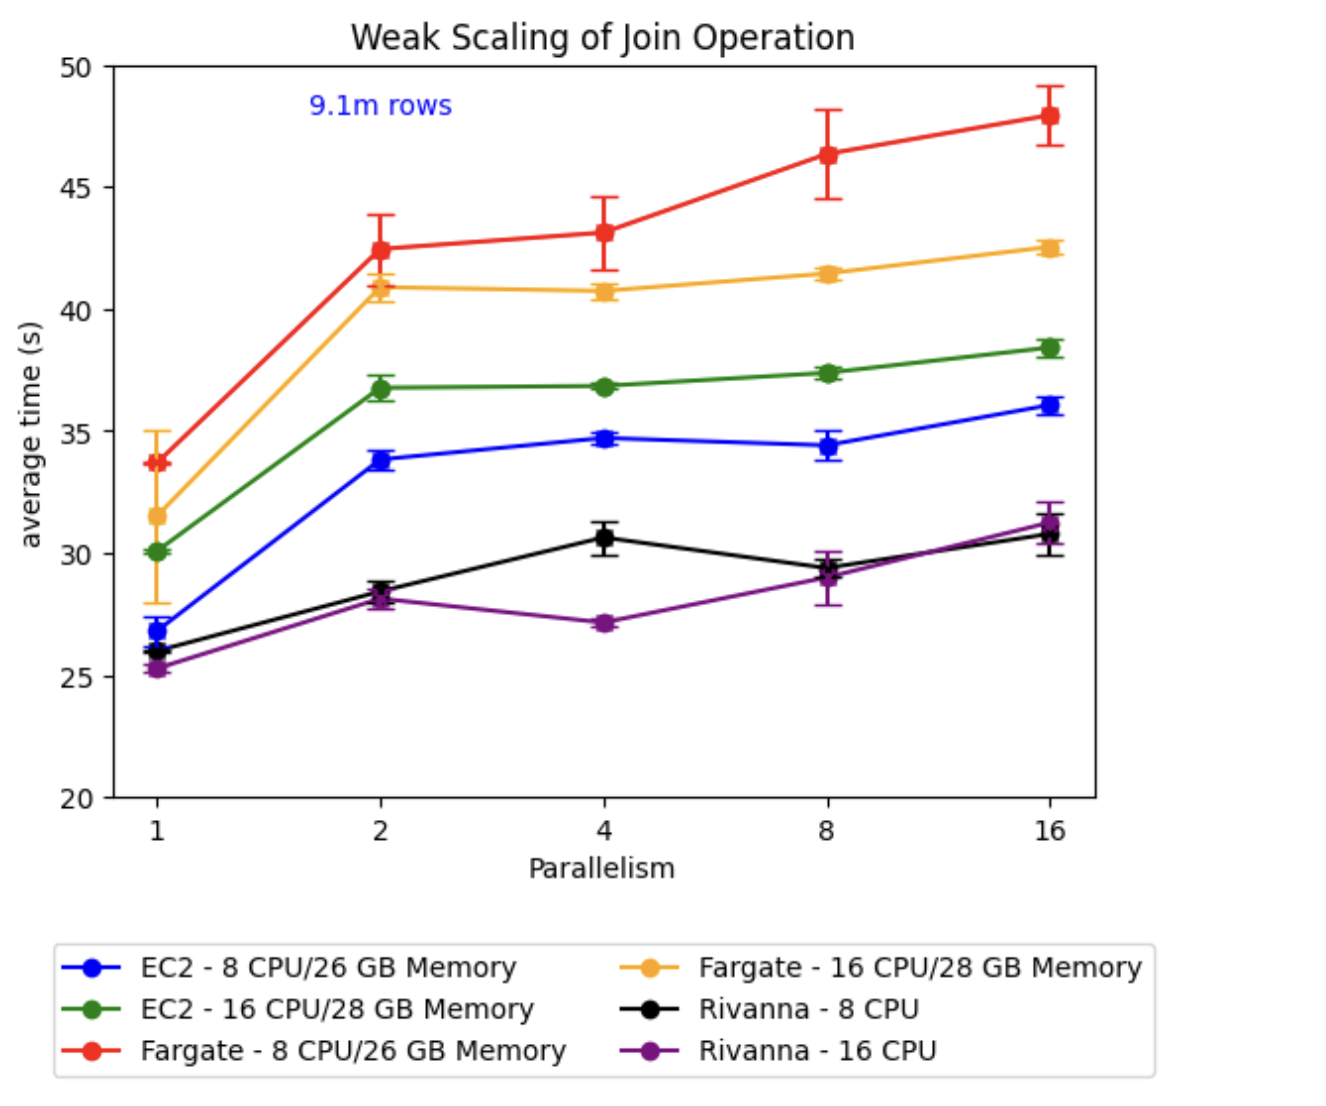
\includegraphics[width=\linewidth]{source/Figure/weakscaling1.png}
    \end{center}
    \caption{Comparison of weak scaling for the Join operation across infrastructure}
    \label{fig:weakscaling1}
\end{figure}

\begin{table}
%\setlength{\tabcolsep}{5pt}
	\centering
	\caption{Execution Time of Strong Scaling from Join Operations Across Infrastructure.}
	\label{tab:strong-exp_table}
	\begin{tabular}{llcr @{\hspace{1\tabcolsep}} lr @{\hspace{1\tabcolsep}} l}
		%
		\toprule
		                   &
		               &
		                     &
		\multicolumn{2}{c}{Execution Time}         \\
	    		%
		Infrastructure             &
		Scaling               &
		Parallelism                     &
		\multicolumn{2}{c}{time (seconds)}                    \\
		%
		\midrule
		\multirow{5}{*}{EC2 8 CPU/26 GB} &
		\multirow{5}{*}{strong} &
		1                       &
		495.40 & $\pm4.75$     \\
		%
		&
		                     &
		2                     &
		302.65 & $\pm2.77$   \\
		%
		&
		                   &
		4                     &
		142.43 & $\pm1.39$    \\
		%
		                    & &
		8                     &
		69.86 & $\pm1.08$      \\
  		%
		                    & &
		16                     &
		35.88 & $\pm0.46$      \\

        \cmidrule{2-5}
    	\multirow{5}{*}{EC2 16 CPU/28 GB} &
		\multirow{5}{*}{Strong} &
		1                       &
		535.91 & $\pm1.40$     \\
		%
		&
		                     &
		2                     &
		308.64 & $\pm2.64$   \\
		%
		&
		                   &
		4                     &
		156.23 & $\pm0.66$    \\
		%
		                    & &
		8                     &
		77.36 & $\pm0.27$      \\
  		%
		                    & &
		16                     &
		38.89 & $\pm0.52$      \\

		\cmidrule{2-5}
    	\multirow{5}{*}{Fargate 8 CPU/26 GB} &
		\multirow{5}{*}{Strong} &
		1                       &
		600.40 & $\pm1.42$     \\
		%
		&
		                     &
		2                     &
		370.67 & $\pm10.69$   \\
		%
		&
		                   &
		4                     &
		190.92 & $\pm7.27$    \\
		%
		                    & &
		8                     &
		92.44 & $\pm2.41$      \\
  		%
		                    & &
		16                     &
		47.68 & $\pm1.11$      \\
		
		\cmidrule{2-5}
    	\multirow{5}{*}{Fargate 16 CPU/28 GB} &
		\multirow{5}{*}{Strong} &
		1                       &
		589.65 & $\pm5.88$     \\
		%
		&
		                     &
		2                     &
		359.92 & $\pm0.76$   \\
		%
		&
		                   &
		4                     &
		173.39 & $\pm0.18$    \\
		%
		                    & &
		8                     &
		85.02 & $\pm0.04$      \\
  		%
		                    & &
		16                     &
		42.71 & $\pm0.0007$      \\

        \cmidrule{2-5}
    	\multirow{5}{*}{Rivanna 8 CPU} &
		\multirow{5}{*}{Strong} &
		1                       &
		328.02 & $\pm1.90$     \\
		%
		&
		                     &
		2                     &
		180.35 & $\pm0.91$   \\
		%
		&
		                   &
		4                     &
		120.38 & $\pm0.66$    \\
		%
		                    & &
		8                     &
		44.00 & $\pm0.61$      \\
  		%
		                    & &
		16                     &
		24.60 & $\pm1.97$      \\
        \cmidrule{2-5}
    	\multirow{5}{*}{Rivanna 16 CPU} &
		\multirow{5}{*}{Strong} &
		1                       &
		442.39 & $\pm1.67$     \\
		%
		&
		                     &
		2                     &
		242.31 & $\pm0.63$   \\
		%
		&
		                   &
		4                     &
		88.91 & $\pm1.03$    \\
		%
		                    & &
		8                     &
		43.80 & $\pm0.54$      \\
  		%
		                    & &
		16                     &
		31.62 & $\pm1.36$      \\
		\bottomrule
	\end{tabular}
\end{table}

Table \ref{tab:strong-exp_table} presents the results of strong scaling experiments involving 145 million rows.  Similar to weak scaling, we conduct the experiment four times, performing ten iterations for each trial.  The results of strong scaling are shown in Figure \ref{fig:strongscaling1}.  We observe high latencies across the infrastructure for fewer than four nodes, and a general convergence of latency as the number of nodes ranges from eight to sixteen.  This supports the validity of utilizing cloud resources as a viable alternative for data parallel preprocessing workloads.  We also assert that cost savings can be realized through cloud infrastructure, given the variable incremental costs compared to the fixed costs associated with traditional HPC clusters.


\begin{figure}[ht]
    \begin{center}
    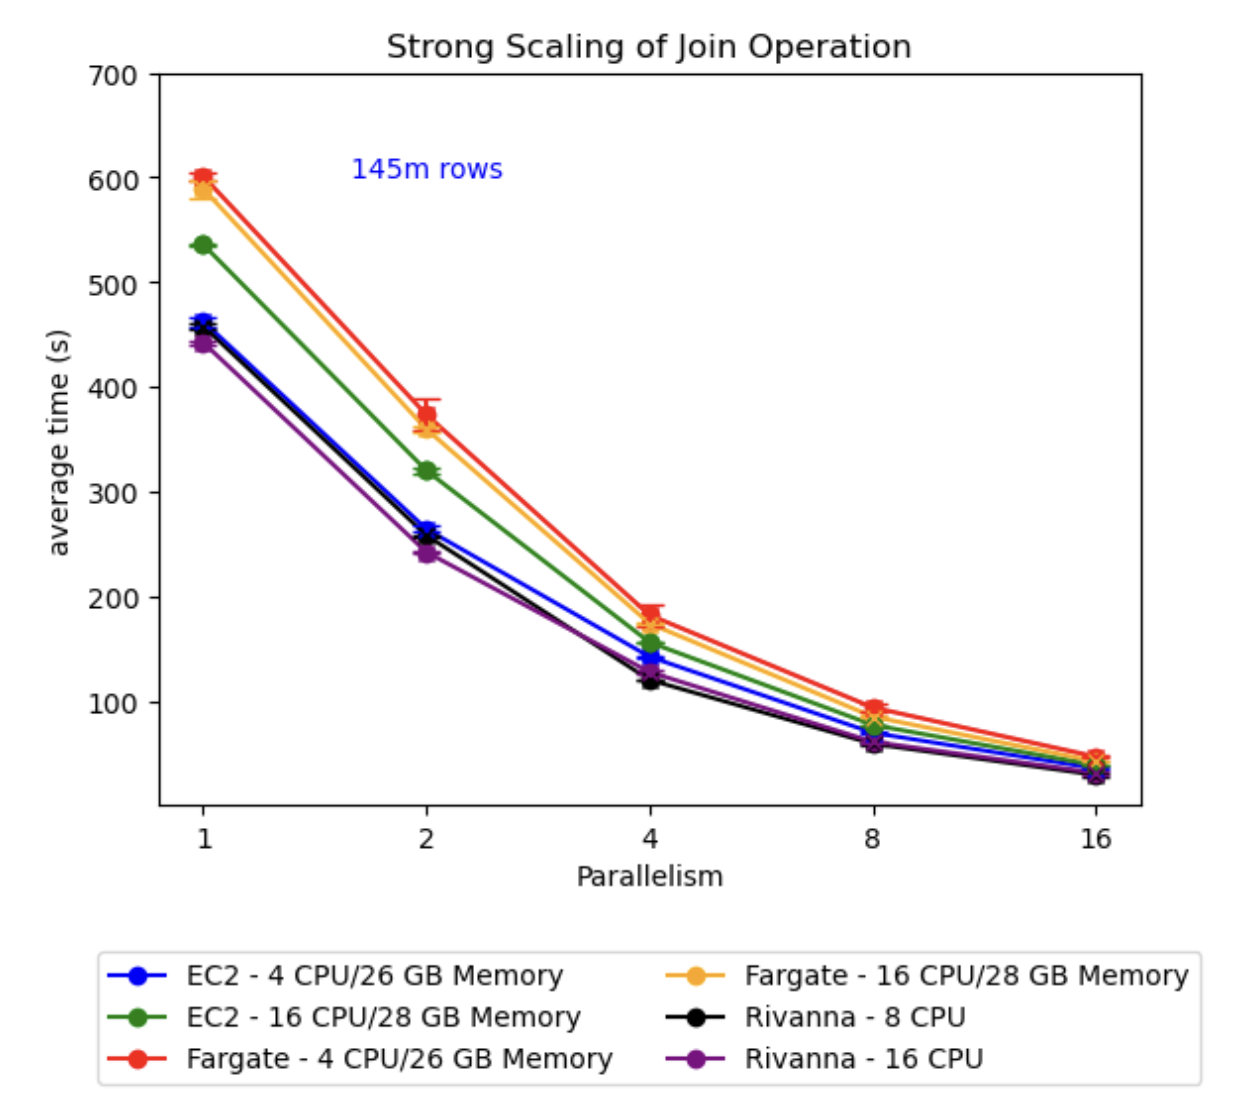
\includegraphics[width=\linewidth]{source/Figure/stongscal1.png}
    \end{center}
    \caption{Comparison of strong scaling for the Join operation across infrastructure}
    \label{fig:strongscaling1}
\end{figure}

We also conducted experiments on one node for AWS and Rivanna with 800000 rows to measure raw performance comparisons of CPUs on those systems.  The number of rows was selected based on memory availability on AWS T2 instances as the lowest common denominator.  We used EC2 (serverful) and Fargate (serverless) Containers on the AWS side.  For  EC2, we used T2 instances, one of the lowest-cost on-demand instance types.  T2 Nano instances (Intel(R) Xeon(R) CPU E5-2686 v4 @ 2.30GHz) were configured with one virtual CPU and .5 GB of memory available.  T2 Micro instances (Intel(R) Xeon(R) CPU E5-2676 v3 @ 2.40GHz) included one virtual CPU and 1 GB available memory.  For AWS Fargate, we used .5 and .25 CPU configurations with 1GB of memory available.  The underlying Fargate hosts used Intel(R) Xeon(R) Platinum 8259CL CPU @ 2.50GHz CPUs.  We executed a similar experiment for Rivanna using the standard partition with one core and one CPU.  Rivanna’s results appear to be three orders of magnitude faster than AWS entry-level instances, presumably based on the processing power of these containers based on the number of rows.  Based on other experiments, we can conclude that as the number of rows increases, Rivanna’s performance begins to converge with AWS weak scaling performance.  The Rivanna host CPU used an Intel(R) Xeon(R) Gold 6248 CPU @ 2.50GHz with forty cores and forty CPUs.  The results of this set of experiments are depicted in Figure \ref{fig:singlenode}.

\begin{figure}[ht]
    \begin{center}
    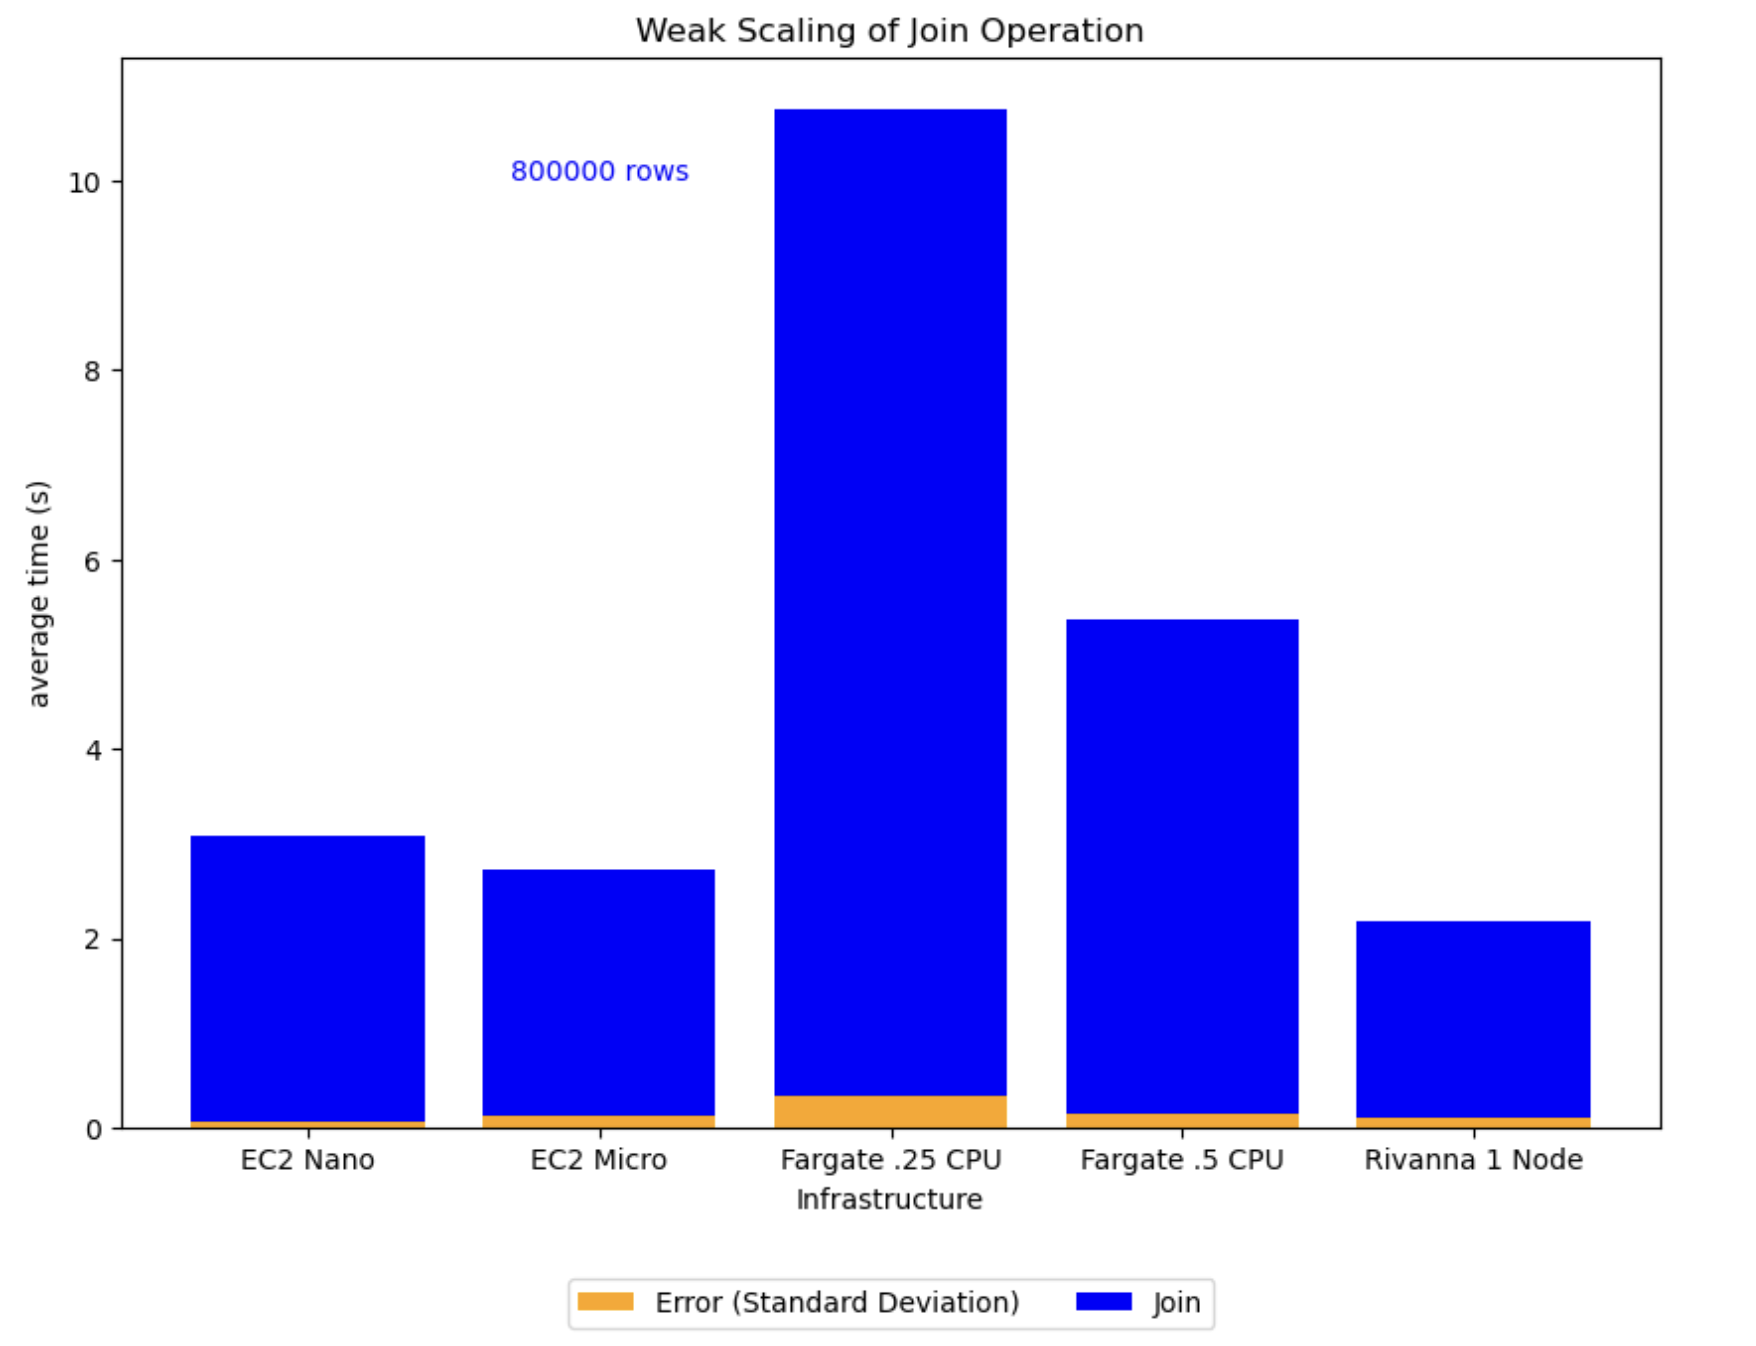
\includegraphics[width=\linewidth]{source/Figure/singleNodeExp.png}
    \end{center}
    \caption{Comparison of weak scaling for the Join operation across infrastructure for a Single Node}
    \label{fig:singlenode}
\end{figure}

For the last set of experiments, we ran scaling experiments plotted as speedup on AWS Lambda, EC2 ECS clusters and Rivanna.  Our intention was to run experiments on derivative configured infrastructure.  For EC2,  we used Ubuntu 22.04.2 LTS (Intel(R) Xeon(R) CPU E5-2670 v2 @ 2.50GHz) for hosts configured with two virtual CPU and 15 GB of memory (m3xlarge) and for hosts configured with one virtual CPU and 7.5 GB of memory (m3large).  For Rivanna, we ran experiments on 1 (standard partition) and 2, 4, 8, 16, 32 and 64 (parallel partition) CPU nodes (Intel(R) Xeon(R) Gold 6248 CPU @ 2.50GHz).  To match the performance and characteristics of AWS infrastructure on Rivanna, we configured experiments that would run on 10 and 6 GB memory configurations.  Rivanna experiments were executed in a Singularity container so that all experiments across infrastructure would be executed using dockerized processes.  For AWS Lambda, functions were configured to use 6GB and 10GB of memory.  Memory configuration influences the CPU available.  For the 6 GB configuration, 4 CPU cores are available, and for the 10 GB configuration, 6 CPU cores are available.  Both configurations use a custom-built AWS Lambda container that includes all the necessary Python and native libraries.  For weak scaling, we used 9.1 M rows, and for strong scaling, we used 4.5 million rows.  The choice of 4.5 million rows was necessary based on memory limitations imposed by AWS Lambda.  Note that additional executions on AWS Fargate (Serverless AWS ECS)  were intended, but changes were implemented by AWS that resulted in breaking the UCX transport discovery mechanism.  In the future, we plan to re-execute experiments using an updated configuration with the FMI library.

For these scaling experiments, we calculate speedup as the execution time ratio to the base case.  The base case is considered the slowest execution or the first node.  Speedup is defined as:
\[
    Speedup = \frac{\text{Baseline Time}}{\text{Parallel Time}}
\]

For the standard deviation or error propagation, we used the following formula applied to the observed standard deviation across executions (i.e., four separate experiments were completed for each node).

\[
    \frac{\Delta{S}}{S} = \sqrt{\left(\frac{\Delta{T_1}}{T_1}\right)^2 + \left(\frac{\Delta{T_2}}{T_2}\right)^2}
\]
\newline
Where:
\newline
\newline
S is the Speedup: S = $\frac{T_1}{T_2}$
\newline
\newline
$\Delta{S}$ is the error in speedup
\newline
\newline
$T_1$ is the baseline execution time (the time for one node)
\newline
\newline
$\Delta{T}_1$ is the error in baseline execution time
\newline
\newline
$T_2$ is the parallel execution time
\newline
\newline
$\Delta{T}_2$ is the error in parallel execution time
\newline
\newline
For these experiments, Figure \ref{fig:weakscalinground3} depicts the weak scaling results, and the strong scaling results are depicted in Figure \ref{fig:strongscalinground3}. 


\begin{figure}[ht]
    \begin{center}
    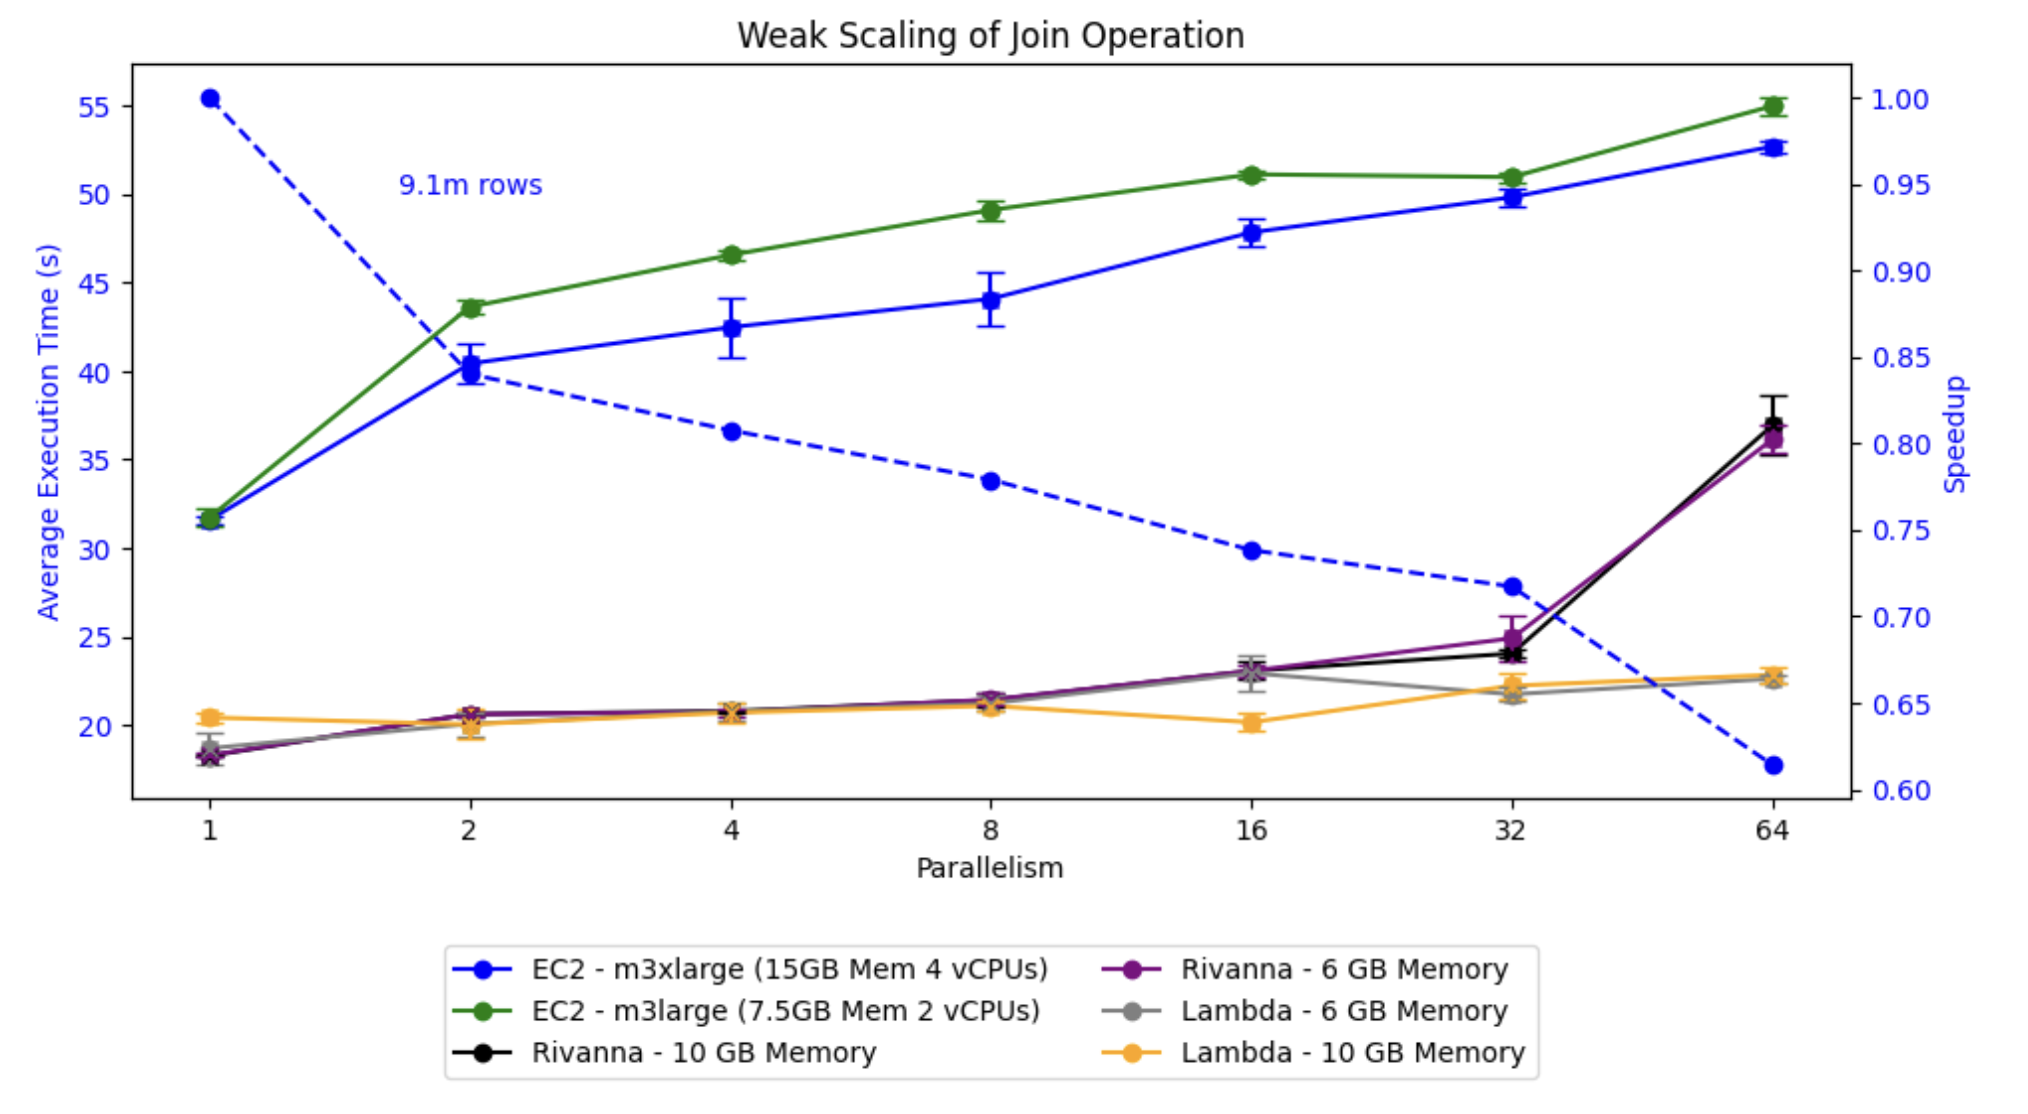
\includegraphics[width=\linewidth]{source/Figure/weekscalinground3.png}
    \end{center}
    \caption{Comparison of weak scaling for the Join operation across infrastructure including AWS Lambda}
    \label{fig:weakscalinground3}
\end{figure}

\begin{figure}[ht]
    \begin{center}
    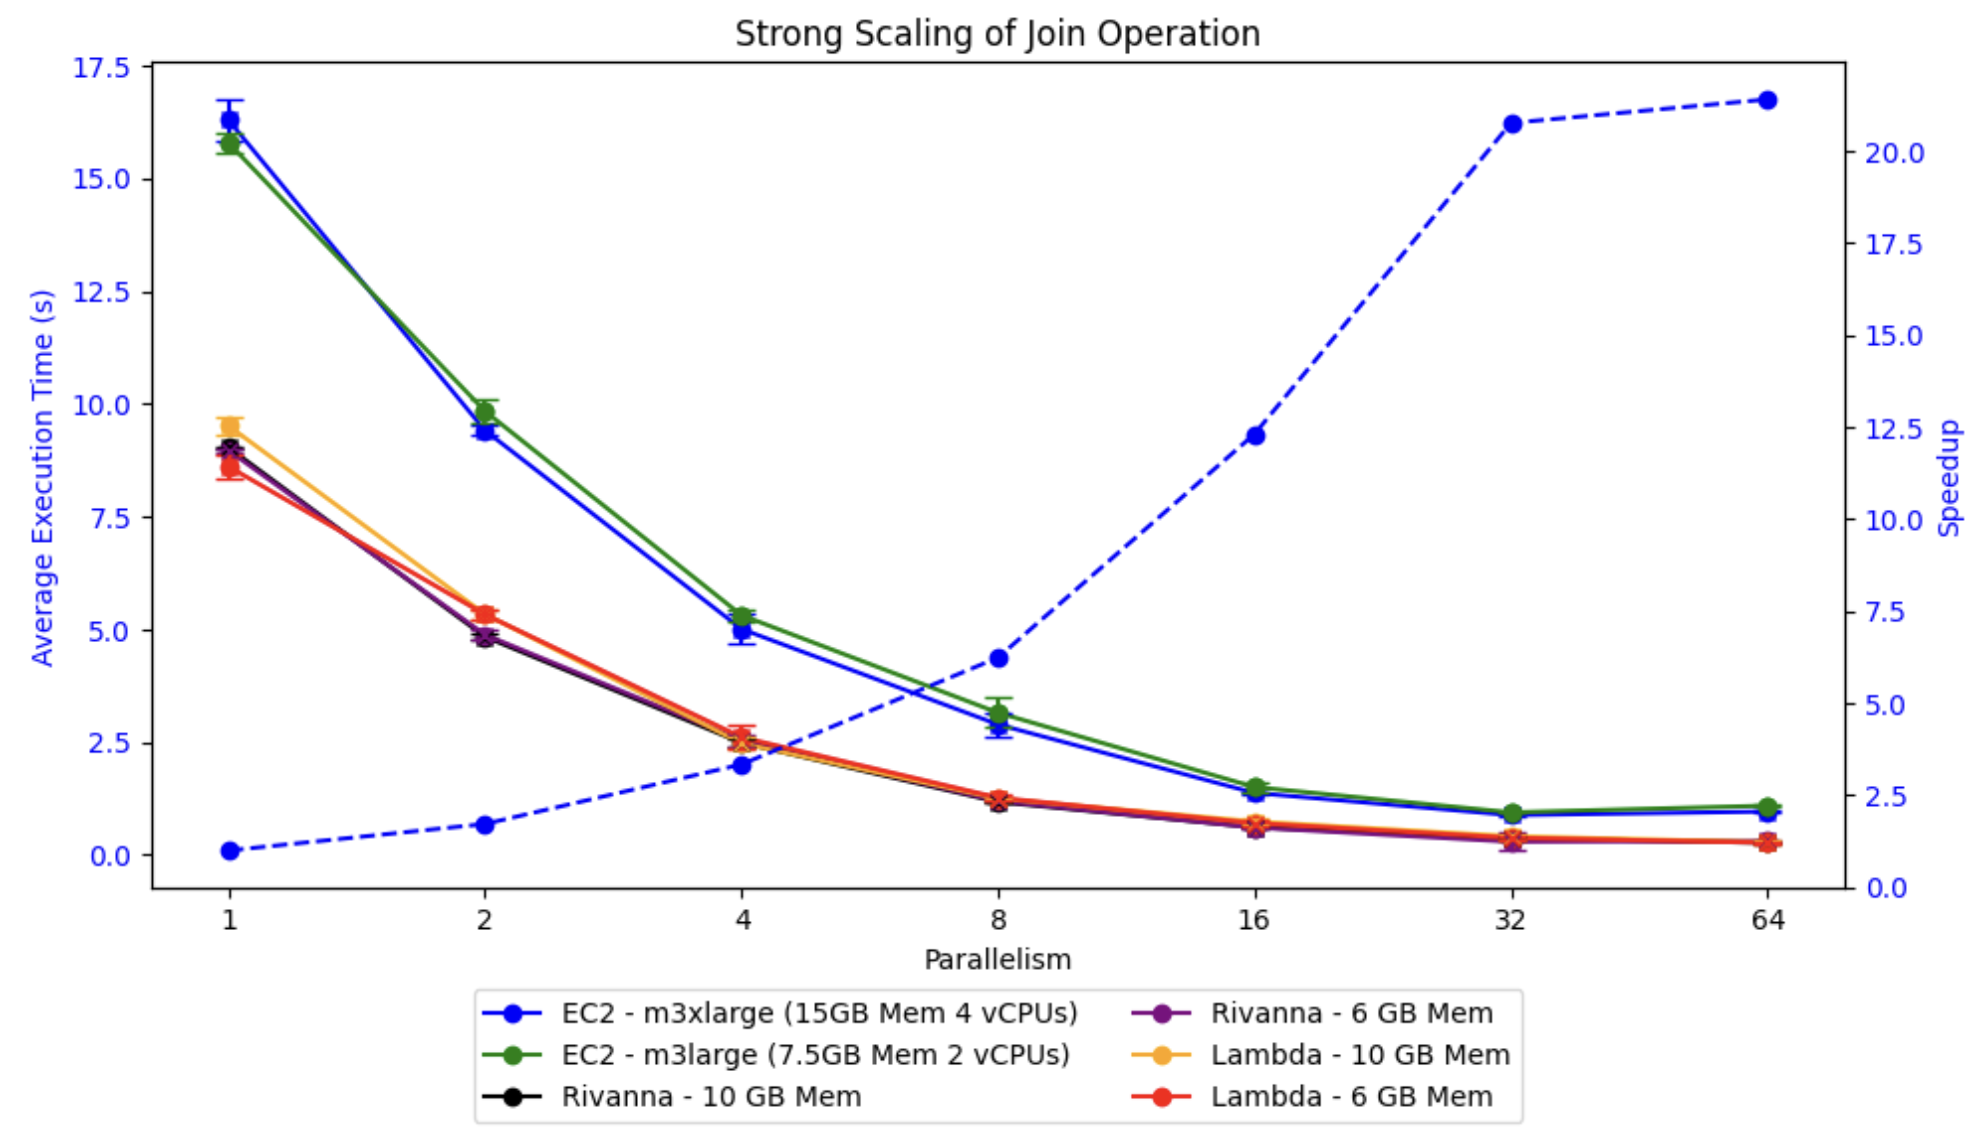
\includegraphics[width=\linewidth]{source/Figure/strongscalinground3.png}
    \end{center}
    \caption{Comparison of strong scaling for the Join operation across infrastructure including AWS Lambda}
    \label{fig:strongscalinground3}
\end{figure}

\section{Future Work}
\label{sec:future}
\textit{Cylon} implements about 30\% of the operators supported by Pandas and we would like to converge Cylon and Panda operators using a comparative, high-performance API built using Cython.  For example, we have begun to implement the windowing operator and plan to complete that work in the near future.  By utilizing the cost model,  we are able to evaluate data parallel operator patterns to identify bottlenecks in communication operations.  We believe we can improve performance significantly by implementing other algorithms that have lower latency\cite{perera2023depth}.  We also plan to complete implementation of FMI as a Cylon communicator.  This will allow us to execute strong and weak scaling experiments on serverless infrastructure such as AWS Lambda and AWS Fargate.  Additionally and related to communicator support, we would also like to add libfabric as a communicator based on implementations across cloud services based on GPU hardware supported by cloud providers.

A key limitation with AWS Lambda is the upper limit of fifteen minutes for a given function invocation.  With a BSP-styled architecture, this limits the applicability of data parallel processing on this infrastructure based on the time required to process large datasets.  This all falls under the subject of fault tolerance.  We would like to implement a similar checkpointing feature is implemented in the Twister2 library.  This will allow for recovery of unfinished executions based on upper limit time constraints imposed by AWS Lambda.  This will also provide general fault tolerance for MPI-workloads outside of the serverless use case.

%In a previous paper, we measured costs associated with Artificatial Intelligence inference on AWS Lambda.  We clearly demonstrated cost savings by leverage AWS Lambda for this use case\cite{Staylor2024cosmic}.  Additionally, our FMI work was used in University of Virginia's Datascience 5110 graduate class.  Costs were significantly less compared to general AWS usage in a previous semester of the same class.  








\section{Conclusion}
\label{sec:conclusion}
In recent years, the growth of artificial intelligence and deep learning has necessitated improvements to data engineering systems to handle the increasing size and complexity of data. We have introduced Cylon, a high-performance C++ library that supports ETL pipelines in Python. Previous papers have highlighted Cylon's superior performance compared to other similar Python data engineering frameworks, such as Abeykook et al.'s paper, "Data Engineering for HPC with Python."  

In this work, we present our integration of UCX and UCC as a replacement for MPI in BSP communication between processes. The novelty of this work is apparent based on a survey of the literature on similar work involving distributed data frames. We applied this work directly and refined the initial implementation to support both serverful and serverless architectures of cloud providers like Amazon Web Services. Additionally, we implemented direct support for Python via Cython, enabling the execution of data engineering tasks in Python without the need to write native code. We also completed the integration of UCC into Cylon by removing our implementation of \textit{AllGatherV} in favor of UCC's support for variable-length data. Furthermore, we implemented container support across infrastructures to facilitate the execution of experiments and library usage.

During the course of this research we encountered a number of challenges that resulted in delays.  We first validated running Cylon on AWS by building the library using AWS Workspaces which was generally successful.   Using AWS facilitated building and running on bare metal because of full control of the underlying ECS host.  Comparatively, building on bare metal on Rivanna was plagued with difficulties based on library changes and security imposed by system administrators for security purposes.  In a related work, RP-Cylon encountered similar delays in months based on challenges building Cylon on Rivanna.  That problem was ultimately solved by addressing fundamental problems with the build to install process.  Later we experienced a similar issue trying to build UCX Cylon after a period of year when updates were applied that broke the previously successful build process.  We were able to solve this problem by using Apptainer or Singularity and running Cylon in a container.  It is our view that use of Apptainer or Docker containers is the future for Cylon based on the inherent challenges associated with building native code on constrained hardware clusters such as Rivanna.

A second problem detailed elsewhere in this paper was related to implementing NAT hole punching within the UCX library.  It was our intention to run Cylon in serverless and serverful environments using UCC/UCX.  The idea was to modify the TCP capability in this library and implement a similar mechanism as what is implemented in the FMI library.  The reasoning behind this choice was FMI shared a similar architecture being developed in C++.  After many months of effort, we were not able to achieve this. 
 We learned and observed the semantics associated with endpoint communication establishment within UCX does not necessary follow the establishment specifics that is required by NAT Traversal techniques.  In retrospect, we believe a fully custom UCX transport would have been an achievable solution.  A key related challenge was the undocumented nature of the UCX library and the complexity of the C code within this library.  Lastly, the device discovery mechanism implemented by UCX uses system level calls to determine the most ideal and optimal communication hardware.  For serverless environments, access to these system calls is prohibited.  This led to the failures executing AWS Fargate experiments based on a change or changes implemented by AWS.

A third problem was related to AWS funding.  We were initially successful receiving funding, but unfortunately research funding expired before we were able to complete our work.  It is an ongoing challenge to perform research on AWS based on the unavailability of AWS as a service by the University and the implicit requirement to apply for funding in order to use cloud providers for research such as what is detailed in this paper.

In this paper, We demonstrated experiments using Cylon and UCC/UCX, comparing them to similar experiments conducted on the Rivanna HPC cluster, to validate the effectiveness and applicability of running data engineering tasks at scale. An emerging paradigm in cloud computing is the use of serverless infrastructure, allowing developers to concentrate on software or applications without the burden of managing infrastructure or other undifferentiated workloads that can be handled by SaaS. We also discuss the challenges of using serverless specifically in communication and present an approach that utilizes NAT traversal through NAT hole punching to enable direct communication between AWS Lambda functions. Additionally, we highlight the relevance of this work to serverless containers such as AWS Fargate and emphasize the significance of architecting communication layers at high levels of abstraction when integrating with serverless compute. We plan to finalize our integration of FMI in the near future and add support for libfabric and checkpoints to facilitate data-parallel execution that extends beyond the fifteen-minute boundary condition imposed by AWS for lambda functions.






\bibliographystyle{ACM-Reference-Format}
%\bibliographystyle{abbrv}
\bibliography{bib/main}

\end{document}